
% \begin{figure*}[!ht]
% \centering
% 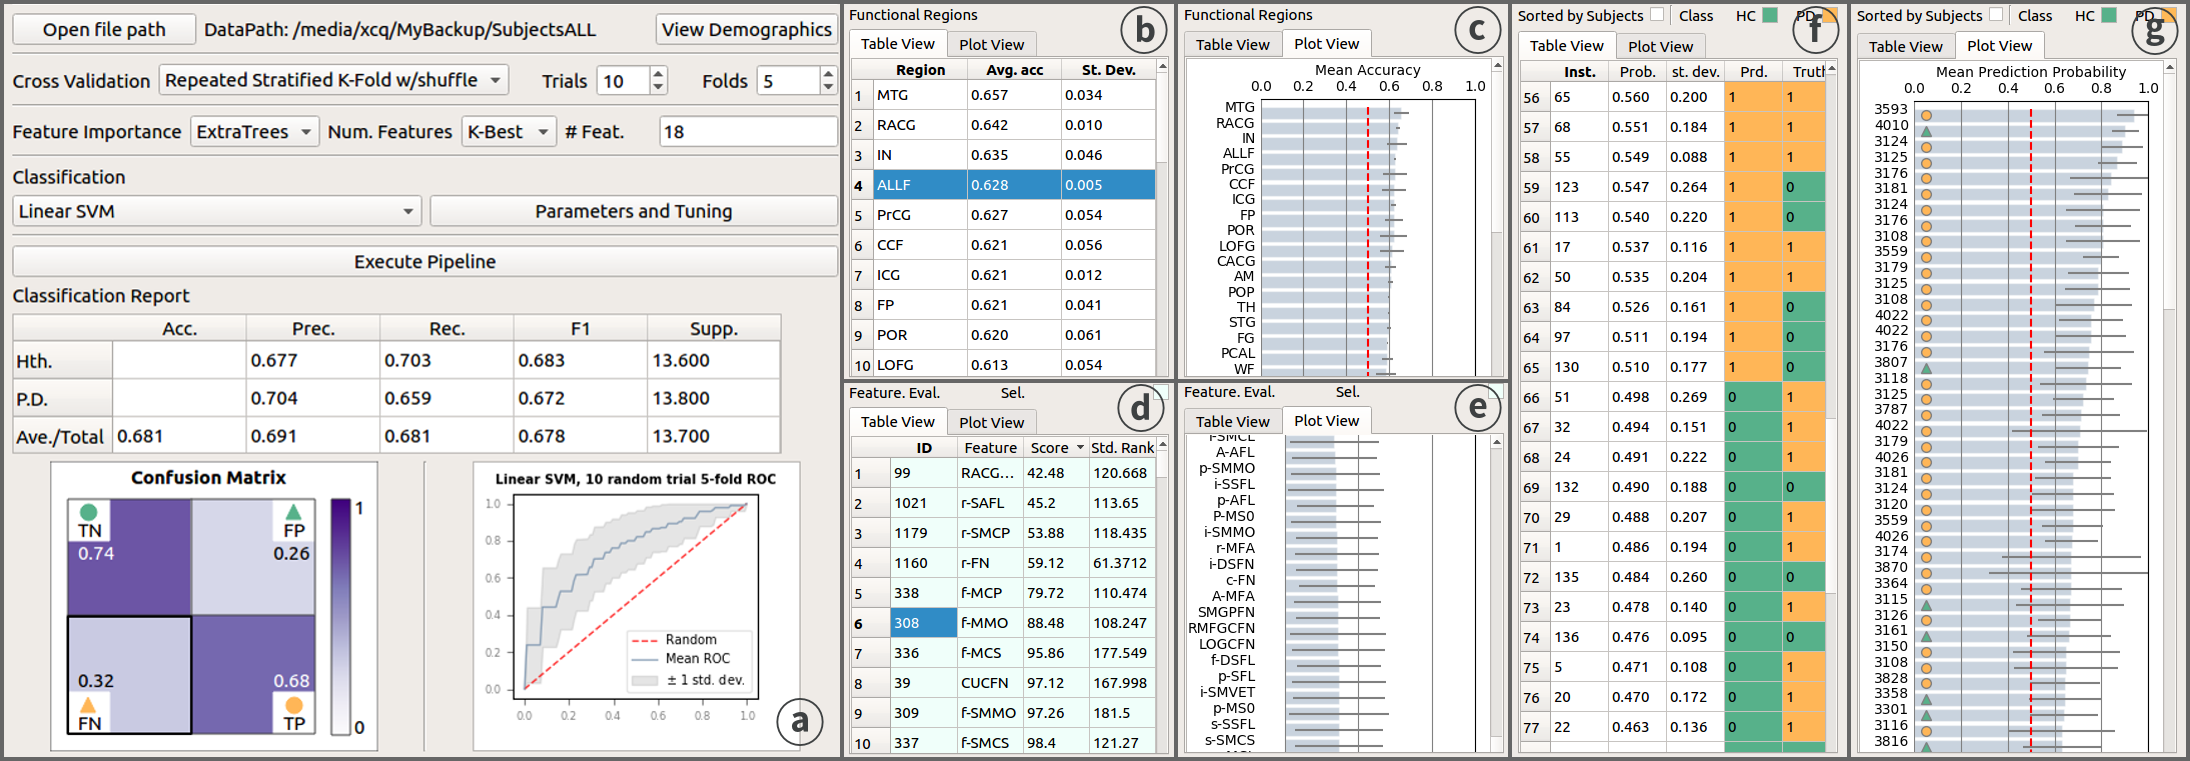
\includegraphics[width=0.9\textwidth]{images/Module_MachineLearning.png}
% \caption{The prediction performance chart in our system. (a) shows the parameter setting for feature filtering, feature reduction, feature ranking and classification. The confusion matrix is shown( left on the bottom), along with the ROC curve(right on the bottom). Brain region ranking and selection are shown in (b), which the regions are arranged in order of accuracy. (c) shows the features that have been ordered by ranking, the top-k highest ranked features have been colored light-blue. (4) shows the subjects that have been ranked according to the predicted probability that they have the disease.}
% \label{fig:MachineLearning}
% \end{figure*}



% \section{ML for Prediction}

% \TF{Many of the parts are not clear if we do not explain the dataset, views, and interactions. So, I suggest that (1) we should explain the dataset in the first subsection (with some description about our system is still desinged for any datasets.) (2) explain each subsection with the corresponding view and interactions. Also, still I don't get it why we want to predict something. (what do we predict? and why do we want to predict it?). Somewhat I understand about the reason, but still it seems not straight forward (i.e., we know the answer, then try to predict PD or not using the selected variables, then find which one is more likely distinguish PD or not. Then, we can more focus on analyze that variable, region, etc.).}.

% \subsection{ Dataset }

% Current dataset contains 140 data, including 69 health group data and 71 disease group data. The demographics of the 2 groups have been compared in Fig.~\ref{fig:demographic}. Due to neurodegenerative diseases are usually age-related, both healthy and disease groups must have similar age distributions. Gender is also within the scope of consideration. In both groups, the amount of male subjects is more than that of the female. "The incidence of Parkinson's disease is low before the age of 50 years, but it increases rapidly with age, peaking in most studies at around 80 years, probably because of underdiagnosis with increasing age" -- this sentence is copying from another article

% Afterwards, we dig out features for each brain data. The features that we obtained fall into 2 categories: tract-based features and tensor-based features. Tract-based features include features based on the number of fibers and fiber length, which are commonly used indicators in brain disease investigation\cite{sundaram2008diffusion}. The tensor based features are the tensor measures calculating from the a diffusion tensor model at each voxel in DTI images, such as Fractional Anisotropy (FA) value, Mean Diffusivity (MD) value and Radial Diffusivity (RD) value, which are widely used in the detection of brain disease\cite{ji2015white}. The whole brain is segmented into 42 regions based on a brain atlas which assigns neuroanatomical labels to each brain functional regions. Fiber tracts and the corresponding tensor measurements are obtained after fiber tracking. Since it has been reported that disease starts from one region and then spreads to other areas, in order to better detect how the disease progresses, we further divided the fiber tracts into 2 categories: inner connect and inter connect fibers. inner connect fibers are fibers in which the start and end points are both located in the same region. Also, since cortical asymmetry and hemispheric predominance have been discovered in neurodegenerative disease \cite{scherfler2012left}, the features `Delta-LR'(the delta value of left brain and right brain) were included to represent the differences between the left and right hemispheres. We calculated those features of different brain functional regions separately. Cumulatively these features amount to about $1,800(42\times2\times14 + 42\times13 + 7\times13 + 4 )$. 42 brain regions, 2 types of fiber tracts (inner connect fibers and inter connect fibers), 14 tensor based features, 13 fiber based features, 7 lobes, and 4 demographics.

% Due to such amount of brain data and each brain contains quite a lot of features, there is a necessity to introduce ML to help identify which features are meaningful for distinguishing the brain disease.

\section{Methods} 
\label{sec:methods}

% The driving mechanism of our system is a predictive modelling pipeline that helps the user identify salient brain regions, fiber tract features, and subjects to prioritize for analysis. This pipeline is integrated as an interface to support intelligently guided VA through those 3 exploration modalities (DG1). The interface is coupled with multiple linked information visualizations and 3D rendering views to support a wide range of comparative modalities (DG3). The comparative modalities and supporting visualizations are chosen to offer a holistic view that provides the context an expert may need to reason about the complex and uncertain information they are presented with. 

\noindent We begin with an overview of our system before going through the detailed design and implementation.

% In this section we describe our methods in detail, and how these different components are linked together to provide a cohesive VA system.

% \subsection{Overview of Our Approach}
\subsection{System Overview}
\label{sec:systemoverview}

% First we give a high level introduction to our system and explain how each of the system components relates to the design goals. 

%\autoref{fig:workflow} 
\noindent Fig.~\ref{fig:system} shows our VA workflow and UI. A preprocessing step includes fiber tracking and feature extraction. In the system, the user begins by selecting cohorts through a module that balances the subjects in each group while stratifying with age and gender (Fig.~\ref{fig:system}\clc{A}). 
%The user then validates the cohort selection by through by opening a view for visual comparison.

Next, the user initiates the ML pipeline depicted in Fig.~\ref{fig:system}\clc{B}. This generates saliency measures for each of the 3 exploration modalities through the following process, repeated for each brain region separately: Through a number $c$ of stratified and randomized $k-$fold cross validation (CV) loops 
%(a method to split the data into different combinations of training and test sets),
%( Sec.\ref{sec:pitfalls})
, estimate each feature's salience based on the training data,  train a classification model based on the top $m$ features, use the trained model to predict the labels of the test data, and record the feature scores, modeling performance (for region saliency), and the probabilistic predictions for each individual subject. 

Afterwards we have $c\times k$ sets saliency scores for each modality; we then compute the averages and standard deviations. The overall modelling performance is summarized in Fig.~\ref{fig:system}\clc{B}, and the saliency scores update the region, feature, and subject exploration modules in Fig.~\ref{fig:system}\clc{C}. As the user explores using these modules, interactive visualization views are generated based on the user's selections, including linked information visualizations and fiber views (Fig.~\ref{fig:system}\clc{C},\clc{D}). 

% The workload is distributed over multiple parallel processes, with each process working on a different region. 

% By increasing $c$, more randomized CV loops are executed (testing more random combinations of test-train data), which will result in better estimation of the uncertainty at the expense of longer wait times to get back the results (see Sec.~\ref{sec:methods}). The process may take several minutes or more depending on number of features, subjects, and CV iterations. 

%This process and workflow provides a solution to our first design goal DG1.


% To support DG2, our system includes a 3D visual comparison view, that can show multiple brains at once with linked camera's. The region that is rendered is automatically selected based on the user's selection from the region importance view. The color mapping of the fibers is based on the feature/variable from the feature importance view. And the compared subjects are based on selections from the subject prediction view. To support efficient, quality rendering, a GPU shader pipeline is used, which includes a geometry shader that converts line data into path tubes, which have an interactively adjustable radius; and screen space ambient occlusion is used to efficiently render lighting with shadows that give better depth perception. These features provide a solution to DG2, and also help support DG3 and DG4. These views are shown in Fig.~\ref{fig:system} \glf{E}.

% Next, as shown in Fig.~\ref{fig:system} \glf{D}, linked information visualizations are used in our system to help support DG3 and DG4. The primary visualizations that are featured in this part of the system include a parallel coordinates view, a specialised scatter plot view that shows the average predicted probabilities of each subject vs their trends in a selected feature, and a group-wise histogram comparison view. The parallel coordinates view helps to support group level comparison of the trends of the top features in addition to comparison of selected individuals features with the group trends. The scatter plot view helps to analyse the relationship between the model, the features, the individual subjects, and the group trends. The histogram view is a simple but useful view, that clearly shows how much overlap/similarity there is between groups in the selected feature. Other visualizations in this module include a correlation matrix and dimensionality reduction. Interactions on these views, the encodings that are used to represent and identify individual subjects throughout these visualizations, and the rest of the system are described in Sec.~\ref{sec:methods}.



% As shown in \autoref{fig:workflow}, brain fiber tracts and their features are collected by the preprocessing step indicated with the red rectangle.
% This step performs fiber tracking on the MRI images including DTI and T1-weighted images, which are commonly used medical image data for brain disease analysis. 

% In order to identify the most effective features and anatomical structures to the disease (DG1), the ML pipeline has been applied for ranking the features, brain regions, and subjects.
% Bases on the predictions, it can produce new hypothesis for researchers in disease exploration. 
% Based on the rankings, the neuroscientist can select specific features and brain regions and analyze relationships across the features, fiber shapes, and disease (DG2) with the information visualizations and 3D fibers. 
% Several linked information visualizations have been provided for showing both of the overall distribution of the features and subjects, as well as showing the relationships between the variables (DG3). 
% In addition to the visualization in population, we also support the comparison across individual subjects. 
% With fiber tracts are rendered side by side in the 3D rendering view and the timeline views of a selected subject, users can intuitively visualize the difference between 2 subjects and observe the progressive changes of a subject.
% Finally, it allows for the verification and exploration of the hypothesis, through the comparative visual analysis of brain fibers and their features in the spatial domain (DG4). 

% Fig.~\ref{fig:system} is the interface of our system that depict how the analytic workflow works.  (A), (B), (C), and (D) show each steps of fiber analysis and exploration, separately. Firstly, all the data have to be loaded and ML methods have to applied to those data. As shown in module (A), researchers are allowed to pick out subjects of certain age range and select classification model for prediction. Secondly, users are allowed to explore the feature that they are interested in according to the prediction results. Module (B) shows the features, brain regions, and subjects that are displayed in a list. Users can manually select the features based on their ranking and prediction for exploration. Thirdly, as shown in module (C), linked information visualizations have been used in our system to show the distributions of the features and subjects. Users can gain an overview of subjects and variables in population. Fourthly, see in module (D), with the 3D rendering of the fiber tracts and the timeline views of the selected subject, users can intuitively visualize the difference between 2 subjects. %users can intuitively visualize the 3D rendering of the fiber tracts with the features mapped to the fiber tracts. Moreover, the timeline views allow users directly visualize the progressive changes of a subject.

\begin{figure}[t]
\centering
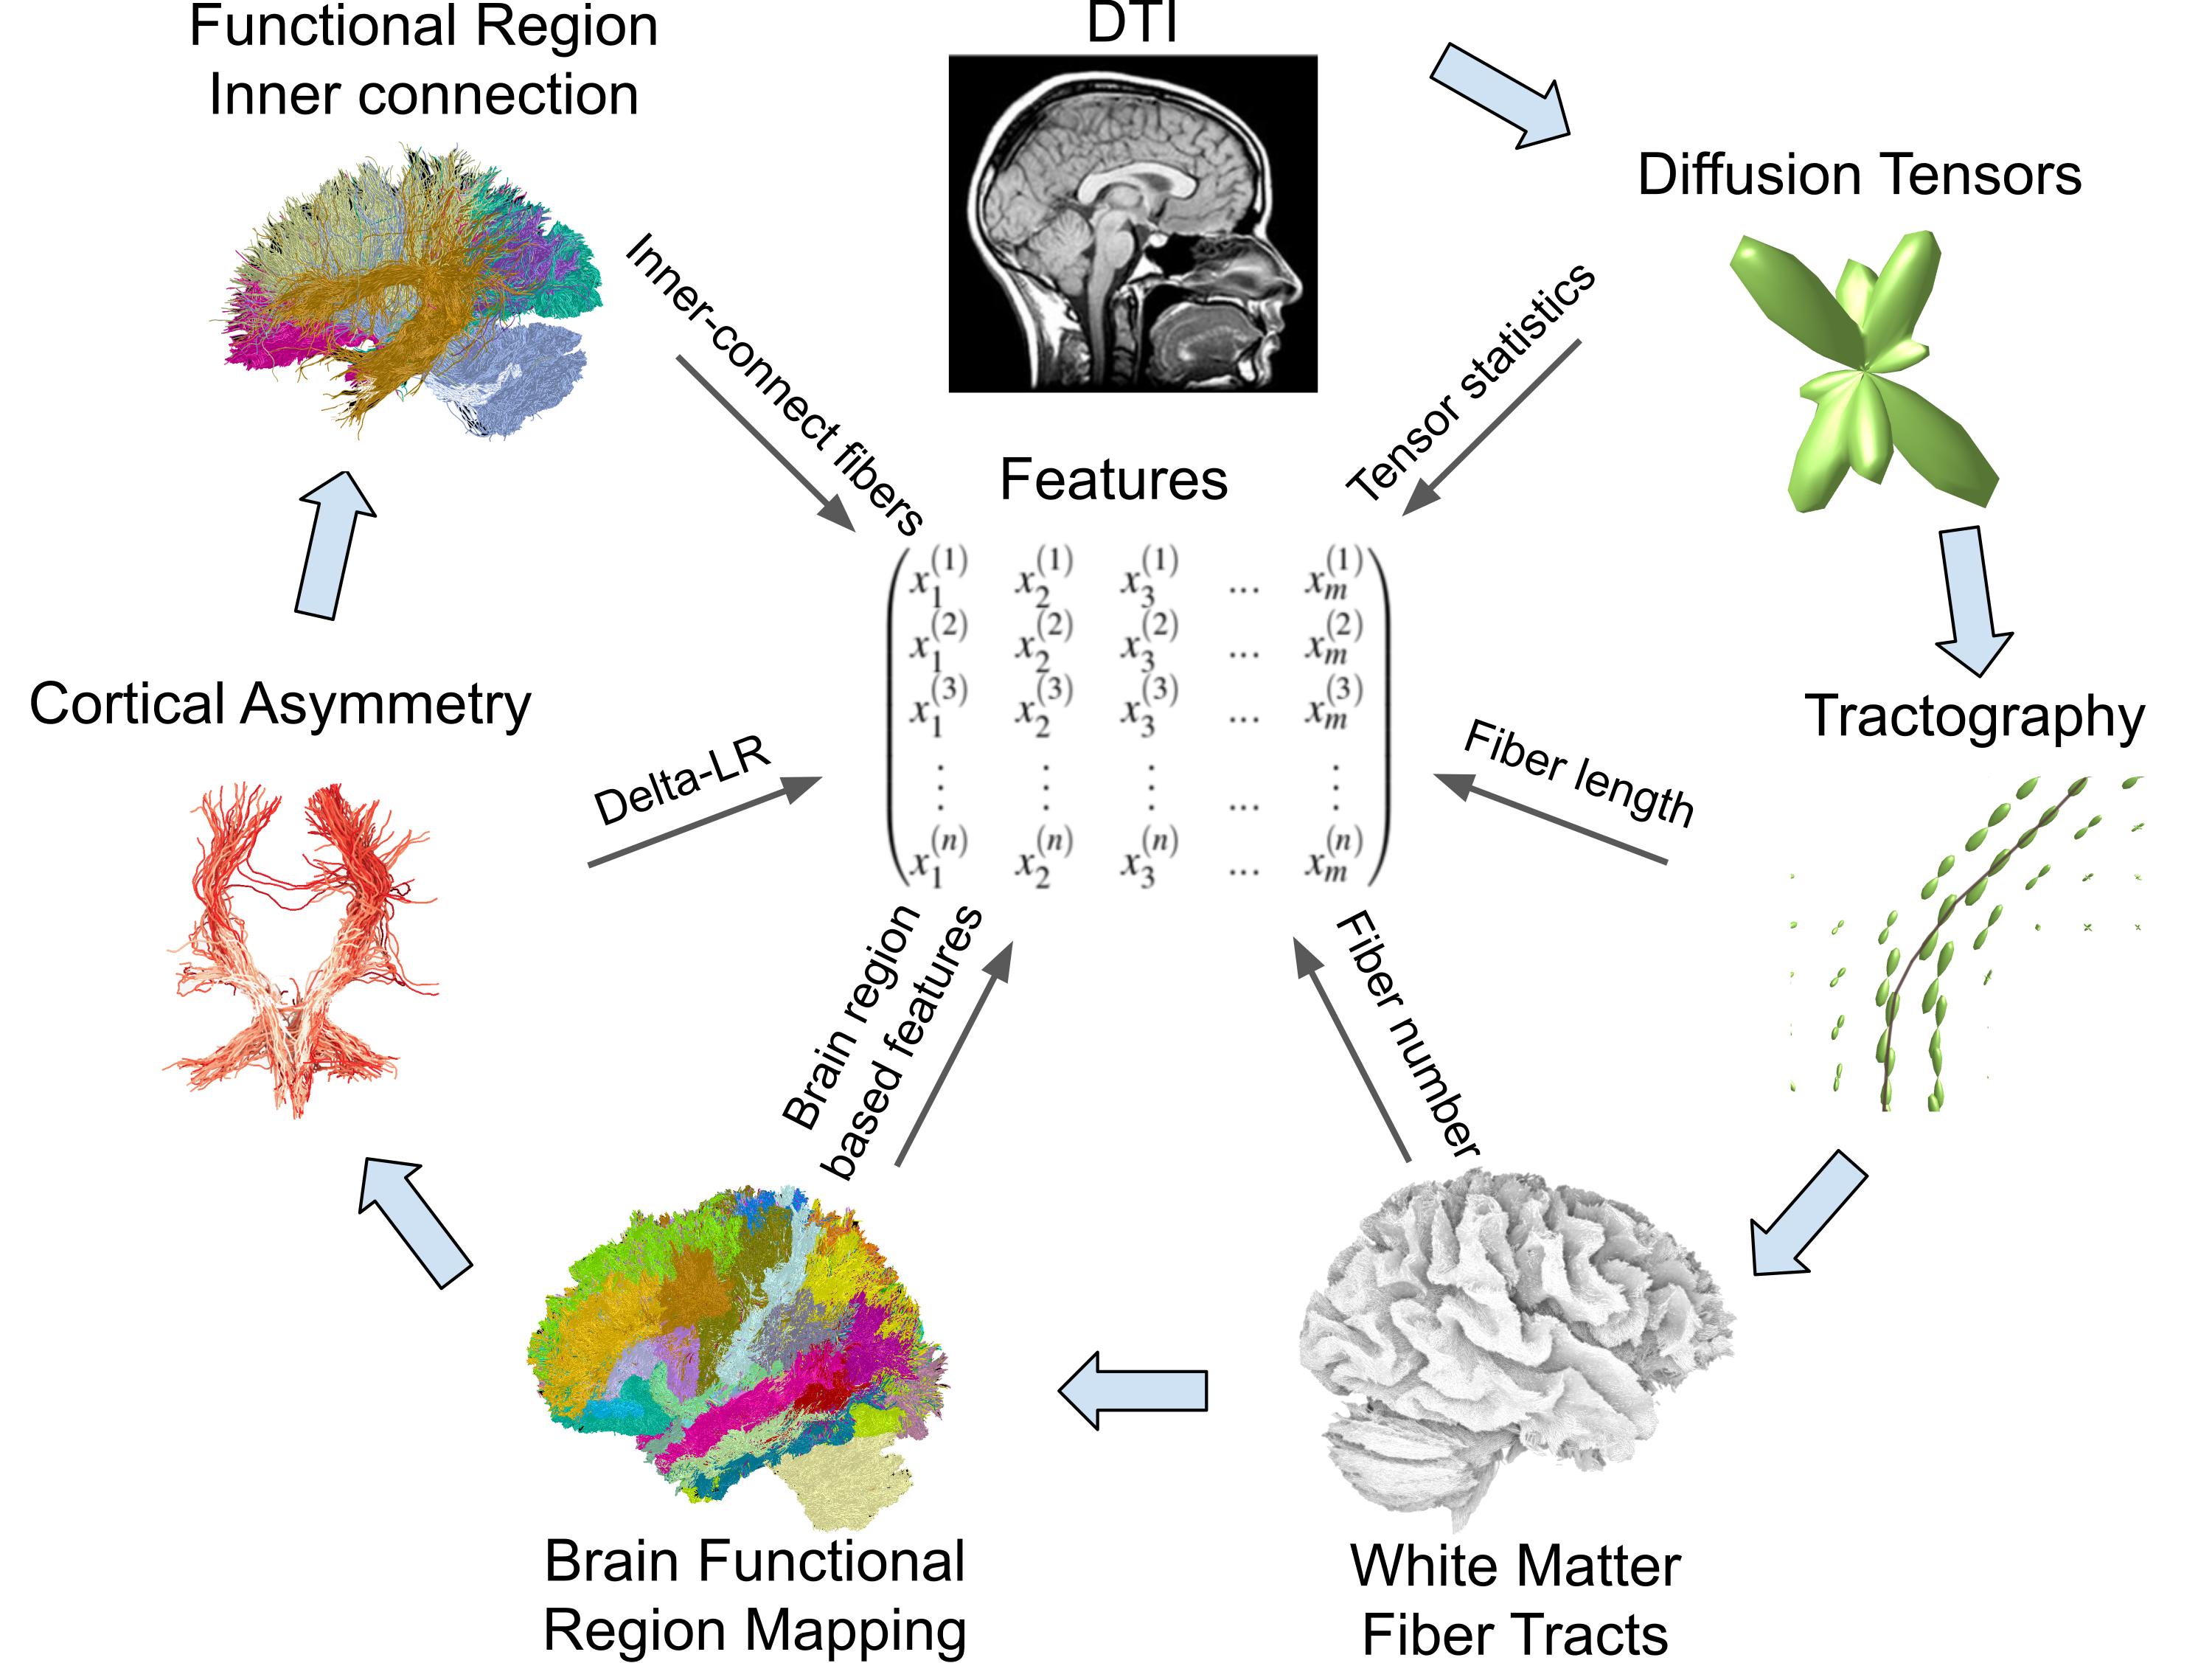
\includegraphics[width=0.95\textwidth]{images/Brainfeatures.png}
\caption{The feature extraction process described in Sec.~\ref{sec:extraction}.
% Feature extraction. White matter fiber tracts are reconstructed from tensors contained in DTI images (which measure water diffusivity). Functional region mapping provides anotomica by the regions. discover the cortical asymmetry of the brain, and show the inner connected fibers of each brain region. The features ranging from tensor fields to fiber tract fields are extracted from each steps of the pipeline.
}
\label{fig:Extraction}
\end{figure}

% \begin{figure}[h]
% \centering
% 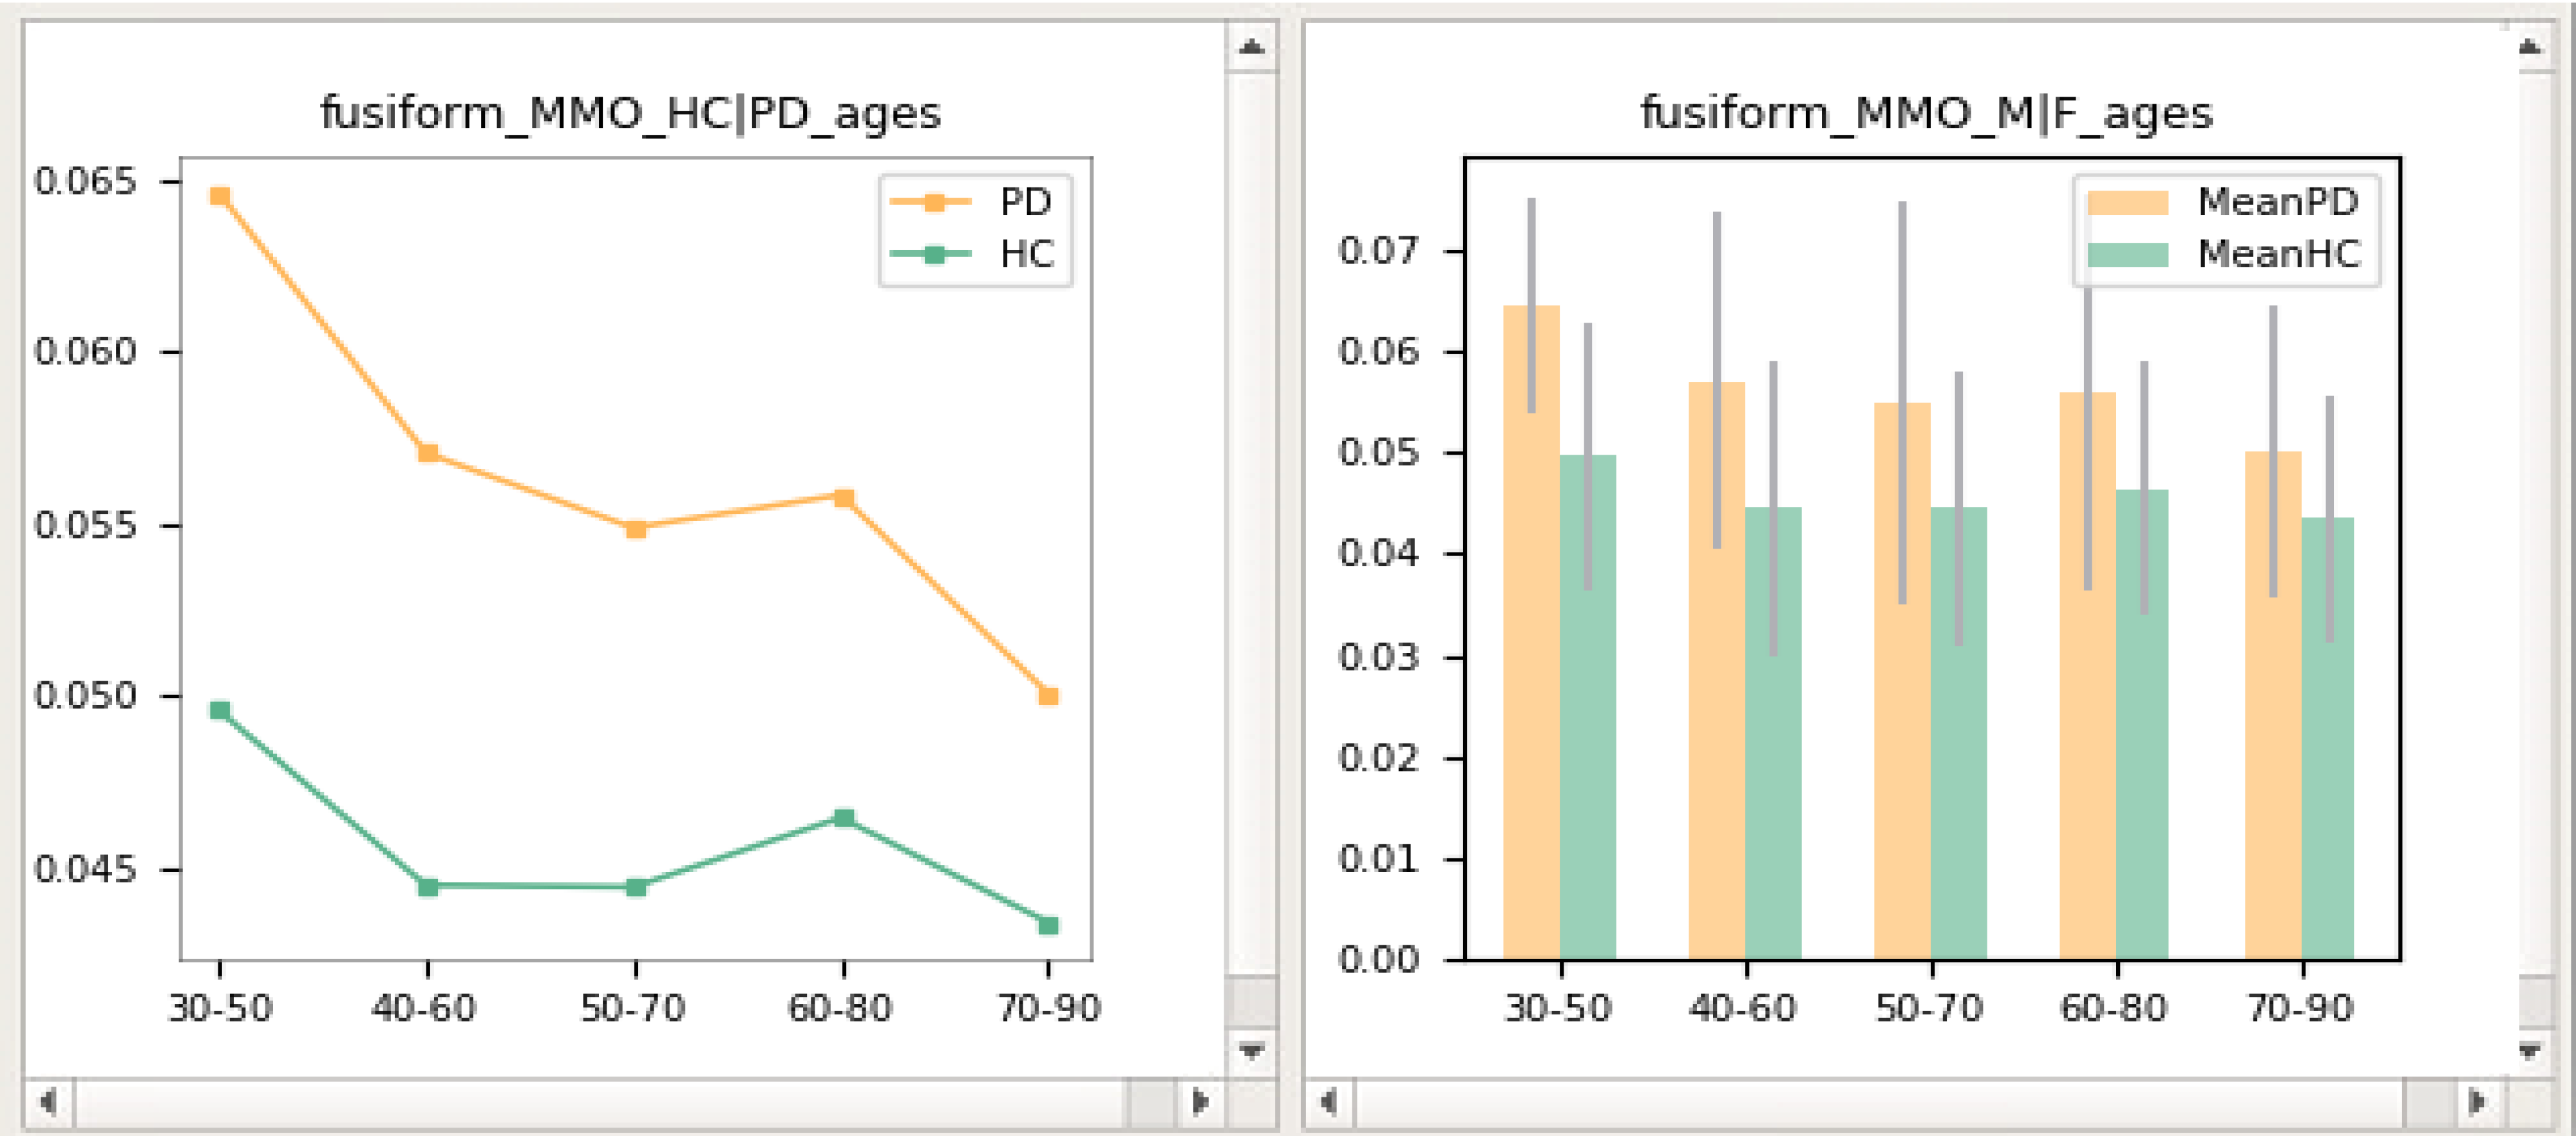
\includegraphics[width=0.85\textwidth]{images/line_Bar.png}
% \caption{Group level comparison of the trends of the selected feature and brain region. The left plot shows a line chart of the MMO feature trends in fusiform region between the 2 groups with age growth, while the bar chart one also aware of uncertainties.}
% \label{fig:line_bar}
% \end{figure}

\subsection{\textcolor{blue}{Data Description}}
\label{sec:extraction}

\textcolor{blue}{In this section, we provide an overview of the data processing: fiber tracking, feature extraction, and cohort formation. These steps are depicted in the preprocessing stage (the left-bottom grey area) of Fig.~\ref{fig:system}. They are not done by the system, and the processed cohort data would be provided to the system. } 

\textcolor{blue}{\textbf{Fiber Tracking}:  The raw data is MRI images (DTI and T1-weighted) from PPMI database. The detailed MRI images description and fiber tractography are described in Section ~\ref{sec:dataProcessing} }

\textcolor{blue}{\textbf{Feature Extraction}}: Afterwards, we extract features using Mrtrix3~\cite{TOURNIER2019116137}. The features fall into 2 categories: tract-based and tensor-based. The former measure regional fiber structure (e.g. density and length), while the latter measure water diffusivity based on a tensor model (e.g. fractional anisotropy (FA) 
%mean diffusivity (MD), 
and radial diffusivity (RD)). Evidence suggests that both categories are affected by neurodenerative disease~\cite{sundaram2008diffusion,ji2015white}.
% Due to the tensor measures are contained in the DTI images, tensor-based features will not be affected by the number of fibers. 

Fibers are bundled based on neuroanatomical labels assigned using a 42 region brain atlas. Also, since PD has been reported to start from one region and then spread to others, 
%features representing connections are worth investigating; thus,
we further divide the bundles into 2 categories: intra-connect and inter-connect (connecting to same or separate regions). Also, since cortical asymmetry and hemispheric predominance have been discovered in neurodegenerative disease \cite{scherfler2012left}, the features 'Delta-LR' are extracted to represent asymmetry between the left and right hemispheres. Tensor-based features are averaged over the different bundles of fibers (Fig.~\ref{fig:Extraction}).

Our choice of features is motivated by literature review and to favor interpretability, follow standard conventions, and support fiber tract based analysis (\textbf{DG1d}). It would also be possible to use dimensionality reduction methods such as PCA and or LDA to derive a reduced feature space. However, the resulting linear combinations may not be readily interpretable. Another approach is deep-feature learning. This may be a good direction for future work, however this would also cause difficulty for interpretation and assimilation. Still, our VA system is decoupled from feature extraction so alternative feature sets can be used easily.

\textcolor{blue}{\textbf{Cohort Formation}:Lastly, we reformulate all the subjects and their attributes, including the extracted features and demographics, as well as their annotations, as cohort data. The cohort data is presented as ".csv" files. Rows represent individual subjects, while columns represent subject attributes. The attributes contains two categories: the whole brain and brain regions. The whole brain attributes consist of suject ID, annotation (binary label: PD or 
HC), age, gender, and visits of scanning MRI. The brain region attributes include the tract-based features and tensor-based features extracted from each brain region according to the aforementioned step.}

\textcolor{blue}{The formulated cohort data is then fed into the ML learning pipeline that includes  feature selection/reduction and classification at multiple levels. All stages were done as described in Section~\ref{sec:MLpipeline}}.

%, however it is important that the features can be rendered in physical space. 

% \subsection{Confounding Factors}

% The first stage of our pipeline involves an analysis and balancing of external factors within the population (e.g. age and gender). Besides balancing these factors between the control and disease classes, understanding the distribution of these factors is important for assessing the uncertainty and limitations of the end results. Therefore, this step is an important preliminary stage, which may also sometimes prompt the user to go back to the data collection phase before proceeding with the analysis.

% Within our UI the demographics are visualized as a pop-up view that shows histograms of the demographics. The view is opened automatically when the analysist first selects the dataset, and can also be opened again manually at any point.

\subsection{\textcolor{blue}{ ML pipeline}}
\label{sec:MLpipeline}

%R1 wants a comparison between the current method and other ML techniques;  R2 wants a figure illustrating the ML pipeline and makes it clearer what exactly is the model and data.  R3 also wants a concrete explanation about how it is used by the experts, what is predicted, which algorithm is applied, and what the training data look like. (It's already in the paper, I guess maybe we should Integrate all these things into a single paragraph?

\textcolor{blue}{ Our system  applies  an  ML  pipeline  that  includes test-train split process and classification. The test-train split process is through the k-fold cross-validation stages in subsection~\ref{sec:CrossValidation}, which is usually integrated in the model training pipeline directly. The classification is established at three levels and we provide the classifier’s performance scores separately in the respective subsections: the feature level (subsection~\ref{sec:featurelevel}),  the brain region level (subsection~\ref{sec:brainregionlevel}), and the subject level (subsection~\ref{sec:subjectlevel}). }
 
\textcolor{blue}{The cohort data is first split into two groups: part as the training set, and the other part as the validation set. As a general approach, we use the training set to train the classifier(SVM), and then use the validation set to test the training model, and estimate the overall performance of the classifier.} 

\textcolor{blue}{Our system integrates a few classical classifiers, such as SVM, Naive Bayes, Logistic Regression, and Decision Tree. etc. In all classifiers, SVM performs best on our dataset. SVM uses the kernel function to map the linearly inseparable data to a higher-level hyperplane space to make the data linearly separable. It is suitable for small sample data in high-dimensional space and is able to handle nonlinear features. It is usually used to solve the binary classification problem, rather than the multi-class classification problem. Such a classifier is very suitable for our data, which contains high-dimensional feature space (1788 features), small sample data (136 subjects), and binary classification (PD or HC). The inherent characteristics of other classifiers limit their adaptability in our dataset. Naive Bayes can efficiently process high-dimensional data, however, it lacks the ability to process data with high correlations between dimensions. Logistic Regression has stronger interpretability for classification results, but with no good performance on large feature space. Moreover, it is a linear classifier and cannot handle the features with high correlations. Similarly, the Decision Tree provided a better understanding of the features in high-dimensional space, but it is easy to cause over-fitting and ignore the correlation between attributes. In addition, Deep learning has also been widely used in medical data, but it relies on a huge training set and is suitable for solving large-scale nonlinear problems. The performance on our dataset would be inferior to classical classifiers.}


\subsubsection{Cross Validation}
\label{sec:CrossValidation}

% {\color{red} proofread up to here: need a simpler explanation of CV, compare with bootstrapping, discuss bias-variance trade-off.}

\noindent Over-fitting a model to a data sample can reduce its ability to generalize to an unseen population. The severity increases with data complexity and limited size. For example, more features creates greater risk that by-chance fluctuations could discriminate target labels~\cite{krawczuk2016feature}. An over-optimized model, learned to exploit those fluctuations, leads to what's called generalization error due to variance. Model simplicity (under-fitting) reduces that error term, but increases what's called generalization error due to bias.
%(e.g. if most $x$ are $y$, then treat all $x$ as $y$). 
The conflict between these two error terms is called the bias-variance trade-off. This issue is an important factor for designing our ML pipeline to support \textbf{DG1e}.

Estimating generalization error (validation), is done by re-sampling into separate test and train samples. Bootstrapping (repeated sampling/testing with replacement), is a good variance estimator, however it tends to poorly estimates bias. Another approach is CV, which samples without replacement. $k$-fold cross validation is a popular variant, which splits the data uniformly into $k$ subsets and rotates their role as the test set $(k-1)$ times. CV gives good estimation of bias, but tends to be sensitive to variance due to a dependency on the partition. Stratification (optimizing representativeness between subsets) helps reduce this sensitivity to a point. Another variant of CV, repeated randomized test-train split, offers an improvement in variance estimation. This has been found to work well compared with $k$-fold CV for neuroimage data~\cite{varoquaux2017assessing}. This makes sense since variance is major problem in neuroimage data due to high complexity and small sample sizes. 

\begin{figure}[t]
\centering
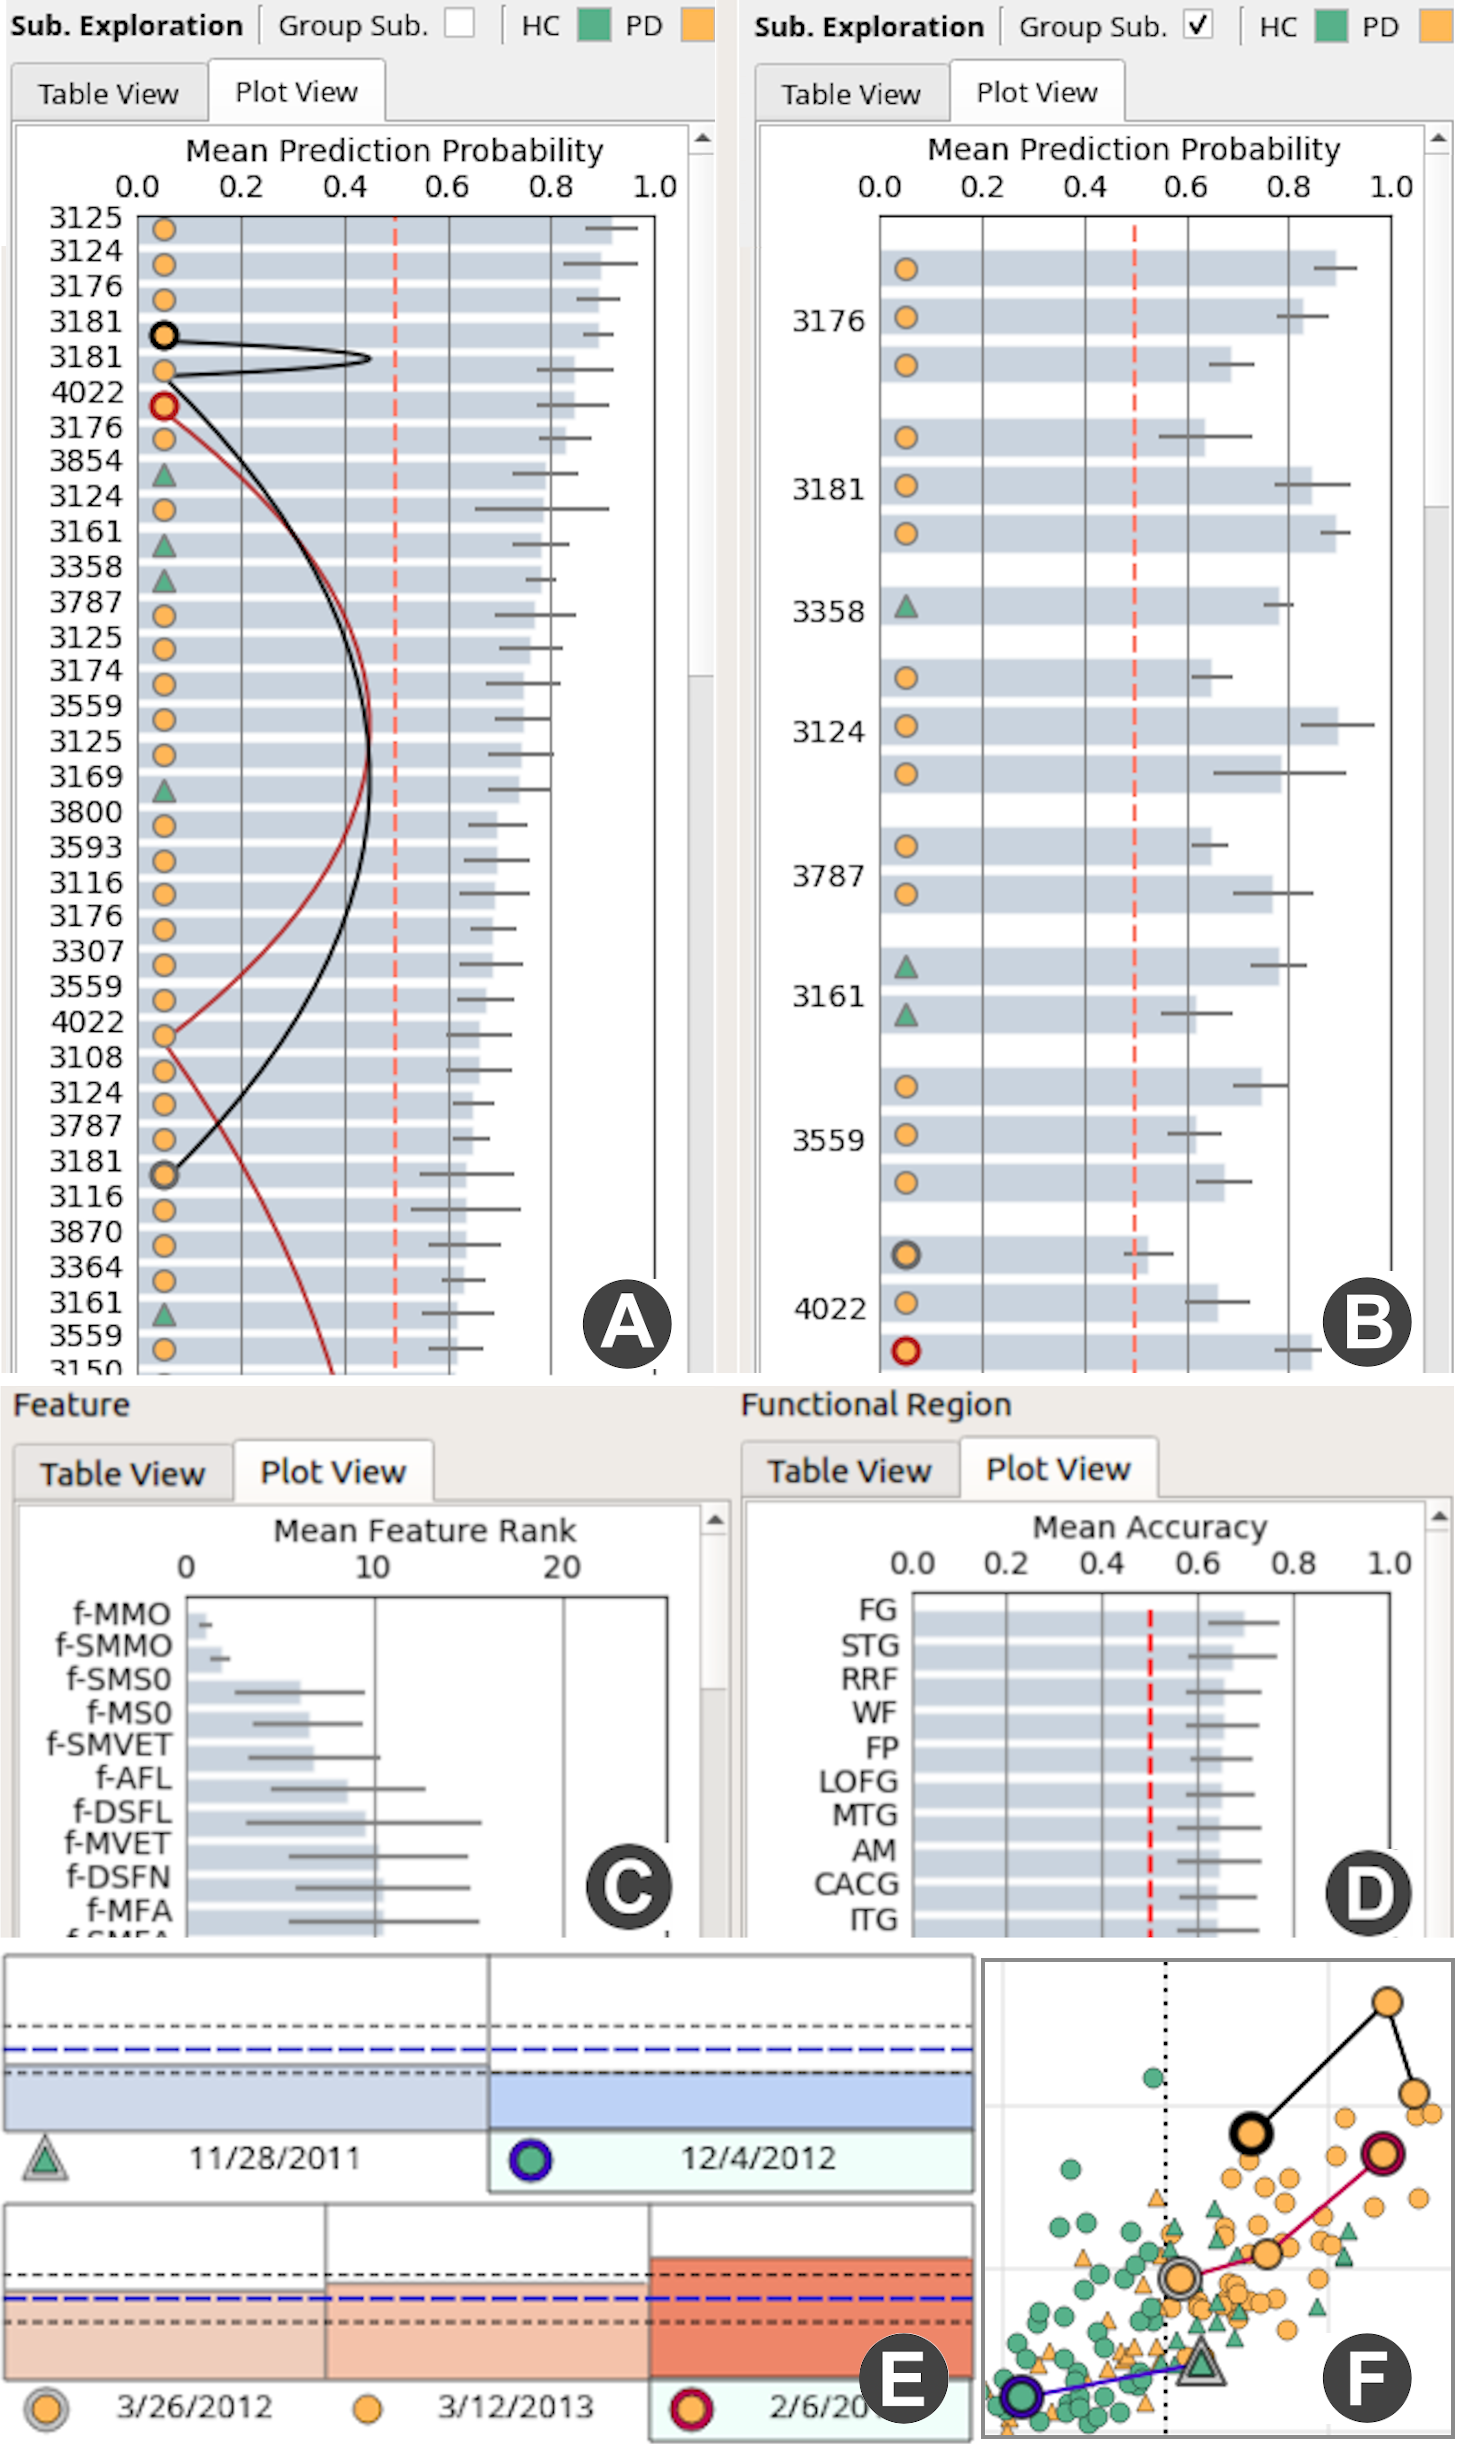
\includegraphics[width=0.95\textwidth]{images/plotView4.png}%
\caption{Plot views of exploration modules and across-view encodings. Glyphs: orange and green fill color encode healthy and disease respectively, circle and triangle encode correct and incorrect prediction, thick borders distinguish compared subjects, their currently selected visits, and which of those visits is the earliest. In this case, dark-blue, dark-red, and black indicate which subject is visualized in the left fiber view, right fiber view, and is mouse hovered in a plot view, respectively. The thick border is colored (blue, red, black) only for the subject's currently selected visit, while their first visit is grey (unless it's selected), and the other's have no thick border. As necessary, lines/curves then connect those glyphs associated with a single subject's multiple visits/scans (\glf{A},\glf{F}), and disambiguate the temporal order. \glf{A} Plot view of subject exploration module sorted by class prediction probability. \glf{B} Same view grouped first by same subject; i.e. their multiple visits are grouped, those groups are then sorted by average prediction, and within group by visit date in increasing order from top to bottom. \glf{C} Plot view for feature saliency. \glf{D} Plot view for region saliency. In plots \glf{A}, \glf{B}, \glf{C}, and \glf{D}, the blue-gray bars encode average score while the thin gray bars encode the standard deviation. \glf{E} The subject time-point selection modules (attached to the fiber views~Fig.\ref{fig:system}\clc{E}) display selected feature over time, and supports switching between those visits. The dotted blue line is the average of the control group, while the black dotted line shows standard deviation.}
\label{fig:subjectsUncertainty}
\end{figure}

One of our objectives is subject level exploration (\textbf{DG1c}) using probabilistic predictions, as described further in Sec.~\ref{sec:subjects}. However, both bootstrapping and repeated randomized CV cannot guarantee that each subject appears in a test set an equal number of times. Standard $k$-fold cross validation does guarantee this, but also may suffer from sensitivity to variance (which is a particular problem in our domain). For these reasons, we use an extension of $k$-fold CV, performed $c$ times with randomization. This allows equal testing of subjects ($c \times (k-1)$ each), and also supports good modelling of the uncertainty/variability. 

Note that choice of $k$ determines the relative sizes of test and train sets at each CV iteration; a smaller $k$ will result in lower representation of the variance in the test-sets, but increased representation of the variance in the training sets. A larger $k$ also results in more overlap in the training sets between each CV iteration. The larger training sets will tend to give a better estimation of the overall performance, and the overlap will tend to cause more consistent between iterations, but in turn may underestimate the variance (giving a false sense of stability). In smaller samples, it's also important that the test sets are representative, which implies a small enough $k$ should be chosen. Ultimately this is a complex trade-off, which is highly data dependent. Based on our goals, the literature, and experiment, we choose a default of $k=5$, which we found to strike a good balance. It can be adjusted within the system based on special consideration by expert users.

% While a smaller $k$ may underestimate the models performance (since less training data is used in each iteration), it may result in more stable estimations that are less affected by variance between test sets (so long as train sets are still representative enough). Erring on the side of stability is desirable for our case, since the data has high-complexity relative to sample size, and our goal is prioritized VA (which benefits more from stable relative saliency estimation than overall performance estimation). 


% One possibility is to separate feature saliency estimation from model training. However, we go against this choice since we aim to also support feature analysis in relation to the classification model in one mode of comparison (\textbf{DG3}). Although it would be possible to include additional saliency measures that have not informed the predictive model, we felt that this may be confusing or easy to misinterpret.

% A popular default for neuroimage data in the literature is $k=5$. For $c$, we use a default of $10$, which is enough to provide strong estimation of the variance, while incurring a reasonable run-time overhead. 
%Besides the outer CV loop, an inner (nested) CV loop~\cite{varma2006bias,varoquaux2017assessing} is used for hyper-parameter tuning and model based feature selection (which require test and train samples that are independent from the outer CV test sets).% Since the inner CV loop splits the training data in the outer CV loop into test and train sets, we must choose a $k$ value for the inner loop as well, and the bias variance trade-off in this inner loop is also affected. This implies a conflict between the benefit of choosing a smaller $k$ in the outer loop (which favors better stability) since if gives less data for the inner loop to work with (acting against stability in the inner loop). 

%Collectively, these choices do well to address \textbf{DG1e}. %Our approach also helps address stability in region and feature ranking~\cite{saeys2008robust} as discussed in the next 2 sections.

% \begin{figure}[!ht]
% \centering
% 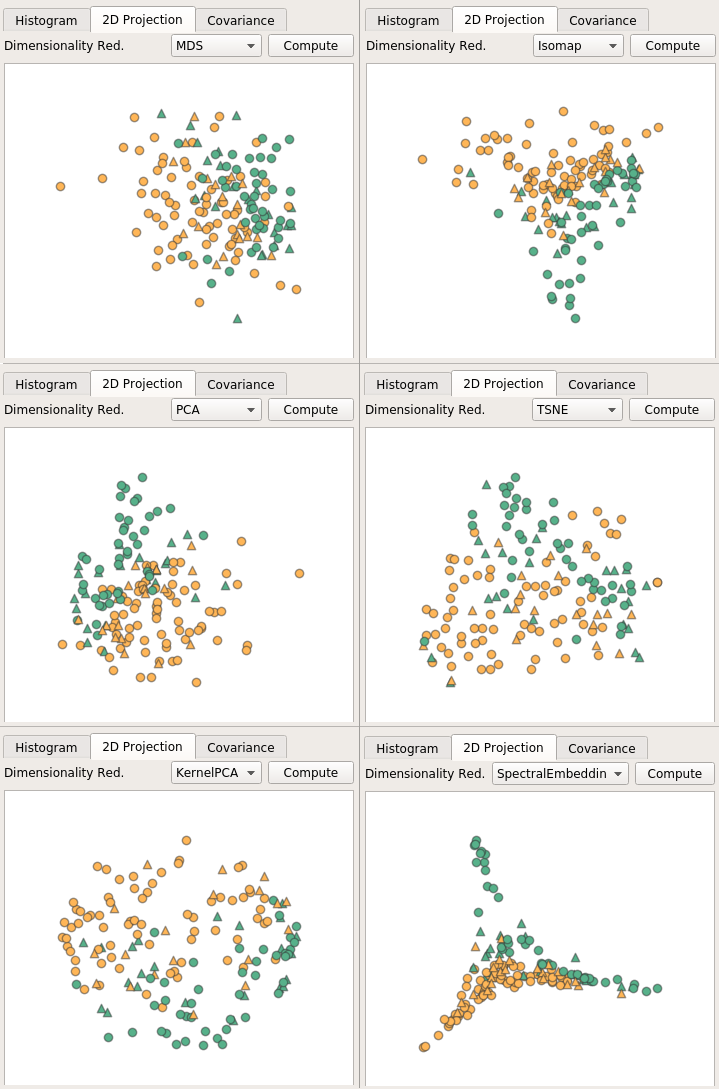
\includegraphics[width=0.9\textwidth]{dimensionalityReduction.png}
% \caption{Our system includes $6$ options for projecting the selected features into 2 dimensions for visualization. Each method appears to work well for separating the 2 groups. Orange shows the disease group, blue-green shows the control group. Triangles represent false prediction, while the circles represent true predictions}
% \label{fig:dimensionalityreduction}
% \end{figure}


% \begin{figure}[!h]
% \centering
% 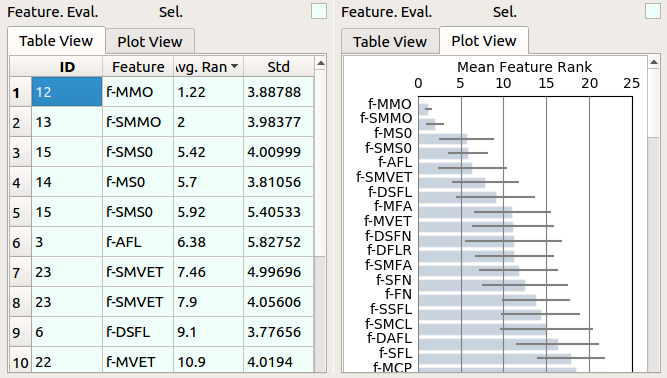
\includegraphics[width=0.9\textwidth]{images/featureRanks.png}
% \caption{ Table view and plot view of the predict features. Table view shows features that are sorted by average ranking followed by standard deviation, while in the plot view bar chart are sorted by the average prediction accuracy and error bars indicate the standard deviation of each feature.}
% \label{fig:featureRanks}
% \end{figure}


% \begin{figure}[h]
% \centering
% 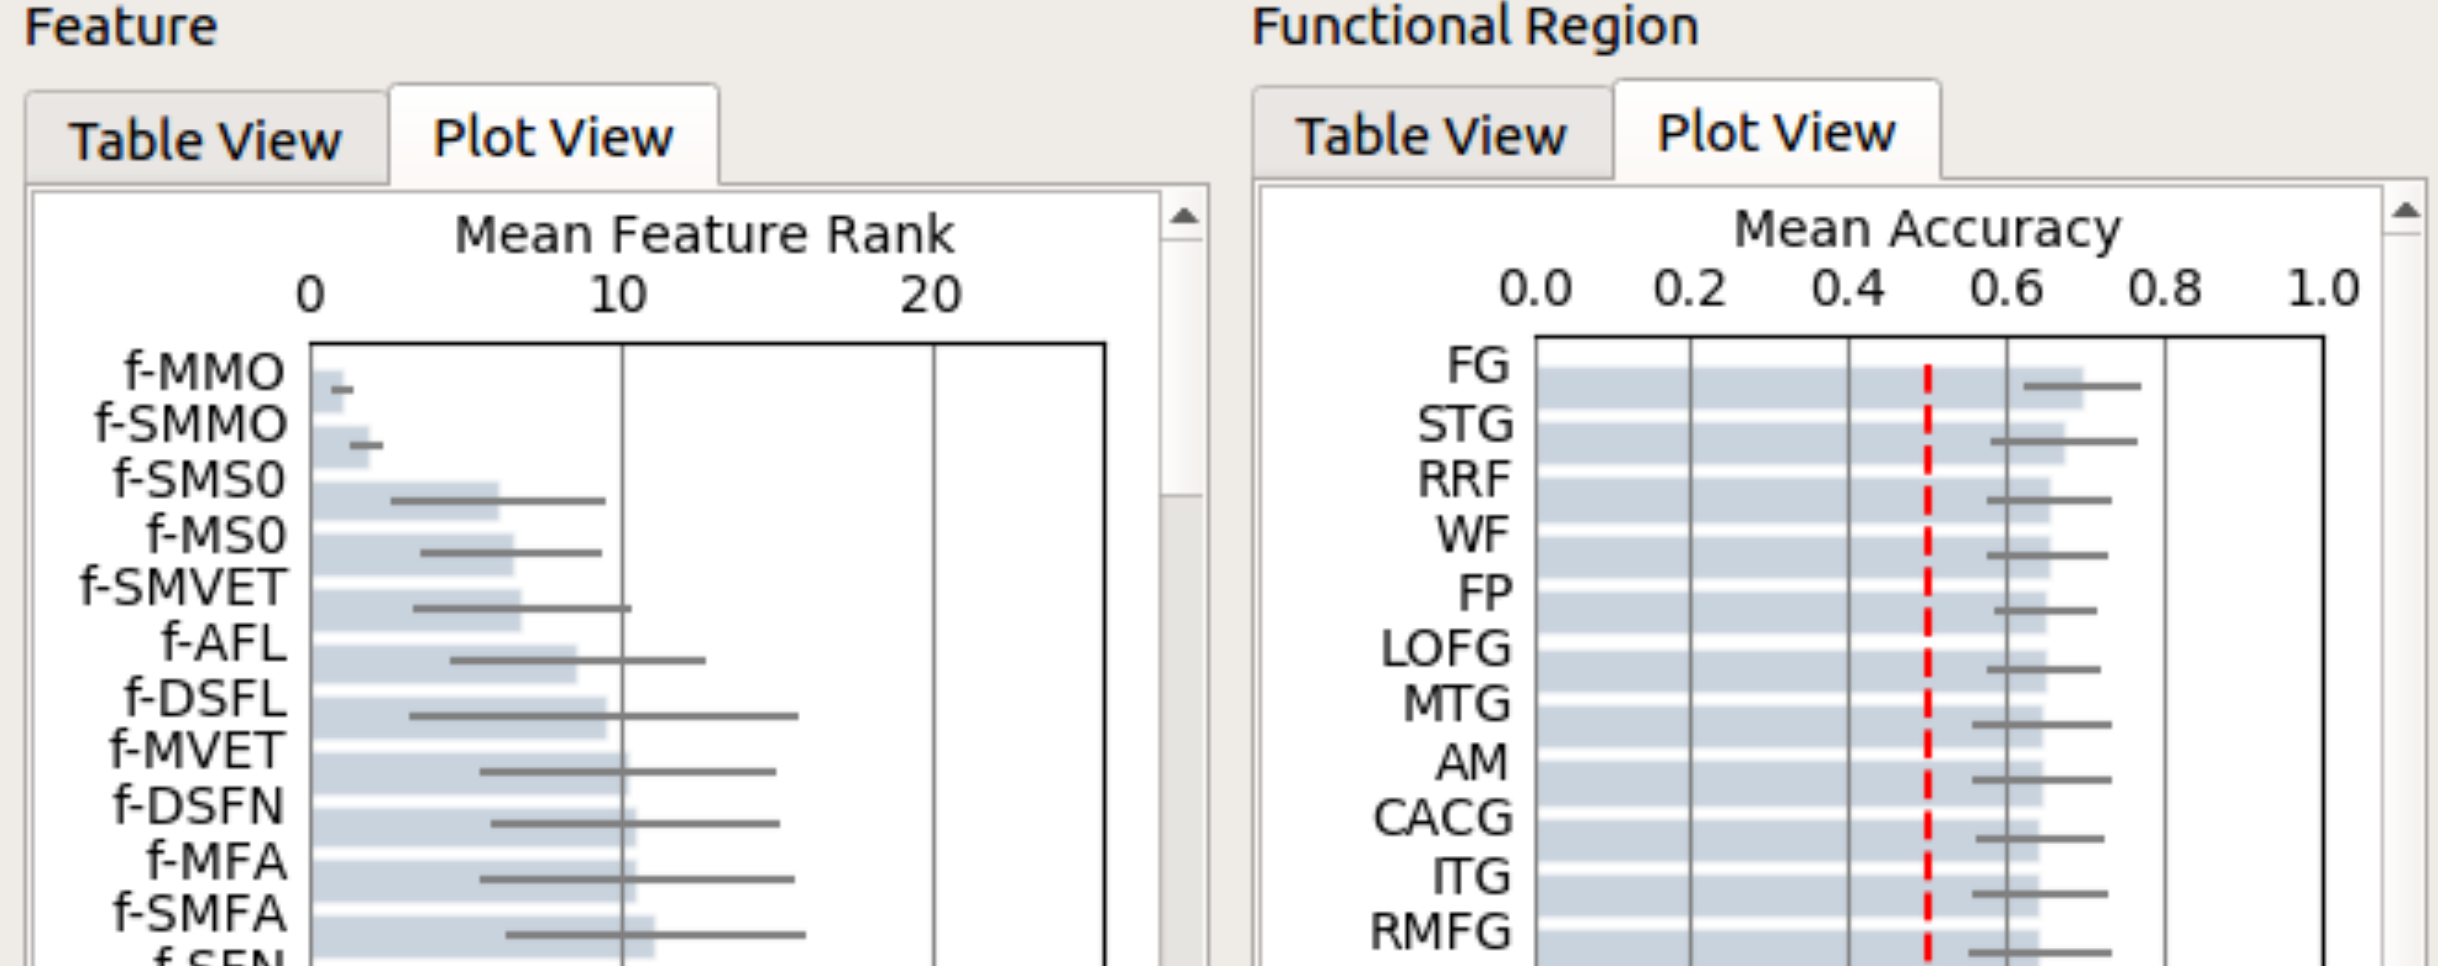
\includegraphics[width=0.85\textwidth]{images/feat.png}%
% \caption{Left)Plot view for feature exploration module. Right) Plot view for module exploration module. Blue bars show saliency score, thin gray bars show standard deviation.}
% \label{fig:regionRanks}
% \end{figure}


\subsubsection{Feature Exploration}
\label{sec:featurelevel}
%  Overfitting is a phenomena where a model fits the training data very well, but fails to generalize (work well on new, unseen data). Typically, the more data you have to train the model with, the better the model will generalize. Furthermore, the feature space is an important factor, and it's relation to the 

\noindent As described, high dimensional data such as ours, suffers from sensitivity to variance. One way to address this is through feature reduction. A rule of thumb is to use between $\sqrt{n}$ and $n$ features, depending on how correlated they are~\cite{hua2004optimal}. One way to reduce the feature space is dimensionality reduction. % as mentioned in~\ref{sec:feature-sel}. 
Instead, we use the given features directly, and discard less useful ones when training the predictive model. There are several possible approaches. A good one is to use statistical significance testing between each variable and the target class since these measures are familiar to scientists and fairly easy to interpret.  Downsides are that multivariate correlations are ignored, and the ranking can fluctuate widely between CV iterations. Another popular but brute force approach is recursive feature elimination, where features are eliminated one at a time if their inclusion in the feature set doesn't improve the CV estimated performance. Problems with this approach are that it doesn't provide saliency scores or rankings that can be used for exploratory analysis, it may keep many features that only slightly improve the performance of the model by random chance, and the run time can be extreme. 

Our objectives (\textbf{DG1}) require saliency scores (ideally stable ones). I.e. the saliencies shouldn't depend too much on fluctuations in the data. Ensemble based methods match these criteria well~\cite{saeys2008robust}. We use extremely random trees~\cite{geurts2006extremely}, a variant of random forests with added levels of randomization to further reduce sensitivity to variance. As mentioned, the features are scored within the CV loops $c\times(k-1)$ times. Finally, the average and standard deviation are used for prioritized VA and uncertainty awareness. In addition, we report \textit{p} values resulting from the Mann-Whitney \textit{U-test} (a non-parametric test of statistical significance) as supplemental information for additional context. The feature scores and their uncertainties populate the feature exploration module as a table view (Fig.~\ref{fig:system}\glf{C}), or a plot view (Fig.~\ref{fig:subjectsUncertainty}\glf{C}). The user can then investigate individual features by selecting them from this view. The selection is automatically linked between the other visualization view described in Sec.~\ref{sec:comparison}. 

% This allows to explore more interactive, subject comparison, as well as investigation of similarities and progression of a single subject's multiple scans over time. 

% Moreover, group level comparison of the trends of the selected features and brain region with respect to ages and genders can be seen in Fig.~\ref{fig:line_bar}. This helps the user to understand how the feature changes with age/gender and the differences between the 2 groups, as well as uncertainty awareness of each group.

\subsubsection{Brain Region Exploration}
\label{sec:brainregionlevel}

\noindent As mentioned, the ML pipeline is performed for each region independently. The averages and standard deviations of the model's performance scores (Sec.~\ref{sec:subjects}) are used for salience based exploration and uncertainty awareness. As with the other exploration modules, these values can be explored in table or plot form (Fig.~\ref{fig:system}\glf{C}, Fig.~\ref{fig:subjectsUncertainty}\glf{D}).

Note that there is a hierarchical relationship between the features and regions. Each region has its own set of features with saliency scores. When a region is selected, all of the other views must update, including the feature exploration module. The fiber bundles for the region are automatically isolated in the 3D views. One design consideration is whether to compute the saliencies for all regions at once or on demand. To make the VA process interactive and support easy non-linear exploration (\textbf{DG4}), we choose to do it all at once. This causes a longer initial wait time, but that time doesn't require user interaction. The whole computation is done in parallel at a process level, with each process evaluating a separate region. When done, the visual exploration process remains uninterrupted as users can switch freely between regions without re-computing. Runtimes are reported in Sec.~\ref{sec:performance}.

%Quantitative performance results are provided in Sec.~\ref{sec:performance}.

\subsubsection{Classification and Across-Subject Exploration}
\label{sec:subjectlevel}

\noindent As explained, the average predicted class probabilities and their standard deviations over all CV loops are used to guide accross-subject exploration. As mentioned, this can help support comparison and hypothesis generation (\textbf{DG3}) in a number of ways, for example: model failure (why some subjects don't fit the model, possible confounding conditions), model success (maybe an obvious case of neurodegenerative expression can be found), model ambiguity (maybe subtle expression can be found through visual analysis, or maybe different features are needed to disambiguate these subjects). In addition, we want to explore the same subjects expression across time. Changes in prediction might help guide clinical analysis and disease progression. 

For classification (to obtain probabilities that each subject has the disease), we use a linear support vector machine (SVM). This model is popular due to its high performance (including with neurological data~\cite{zhang2015detection,dinov2016predictive}), robustness against over fitting, and ability to return class probabilities (rather than just binary predictions). All of these qualities make it a good model for our domain and the objectives stated in \textbf{DG1}. 

% As the performance scores are used to rank regions, we must choose a classification performance metric.  The system reports accuracy, precision, recall, and $F_1$. We found with our data that each metric was consistently very similar in value. By default, sort by $F_1$ (which incorporates precision and recall into one score), but note that for unbalance data another metric might be preferable. 

Also, as mentioned in \textbf{DG3}, we aim to facilitate a wide range of subject-level comparative analysis through linked visualization views. First, we need to highlight/distinguish points representing multiple selected/compared subjects in each appropriate view. One complication is that there are multiple scans/time-points for each subject. In addition to highlighting and distinguishing compared subjects, we also need to associate and select between same-subject time-points and disambiguate their temporal orders. In addition, besides encoding which class the subjects belong to (disease,healthy) it's helpful to encode which class the model predicted. The subject exploration view, and these encodings are demonstrated and explained in Fig.~\ref{fig:subjectsUncertainty}.

% The ability to select individual subjects for fiber rendering based on their predicted probabilities and true values supports a useful means for exploring the variations of physical features. For example, one might expect that the more strongly effected disease brains would be predicted with a higher probability, and thus by selecting them we can see the most severe cases. By selecting lower and lower probability predictions, we can then expect to see progressively more affected subjects. Finally, we can expect that the false predictions are more likely to be outliers, and are potential indicators of bad data, for example, from imaging or processing errors, that need to be pruned out.

% As shown in Fig.~\ref{fig:subjectsUncertainty}, the probabilities and uncertainties of the subjects predicted of having PD are visualized as a sorted bar charts that include the standard deviations. The user can then investigate individual subject prediction trend and the uncertainties.

% The system supports comparison between different subjects in juxtapositioned views. The compared subjects are highlighted in the partial dependence plot and the information views, and their fiber tracts are rendered side by side in the 3D rendering views. 

% Finally, since each subject may have had their brains scanned several times over several years, when one of their scans is selected, we highlight their other scans in each of the point based information visualization views. Lines connect them while the border color of the glyph is used to indicate the currently selected time step, differentiate the different compared subjects, and help indicate the temporal order. In addition, the filled color of the glyph indicates the true class, while the shape indicates true or false prediction (circle and triangle, respectively). Additionally, we show their timelines within the fiber rendering view, with their mean values of the selected feature over time. This timeline can be used to select the subject's other scans. These views and the associated encodings are illustrated in Fig.~\ref{fig:encoding}.

% \begin{figure}[h]
% \centering
% 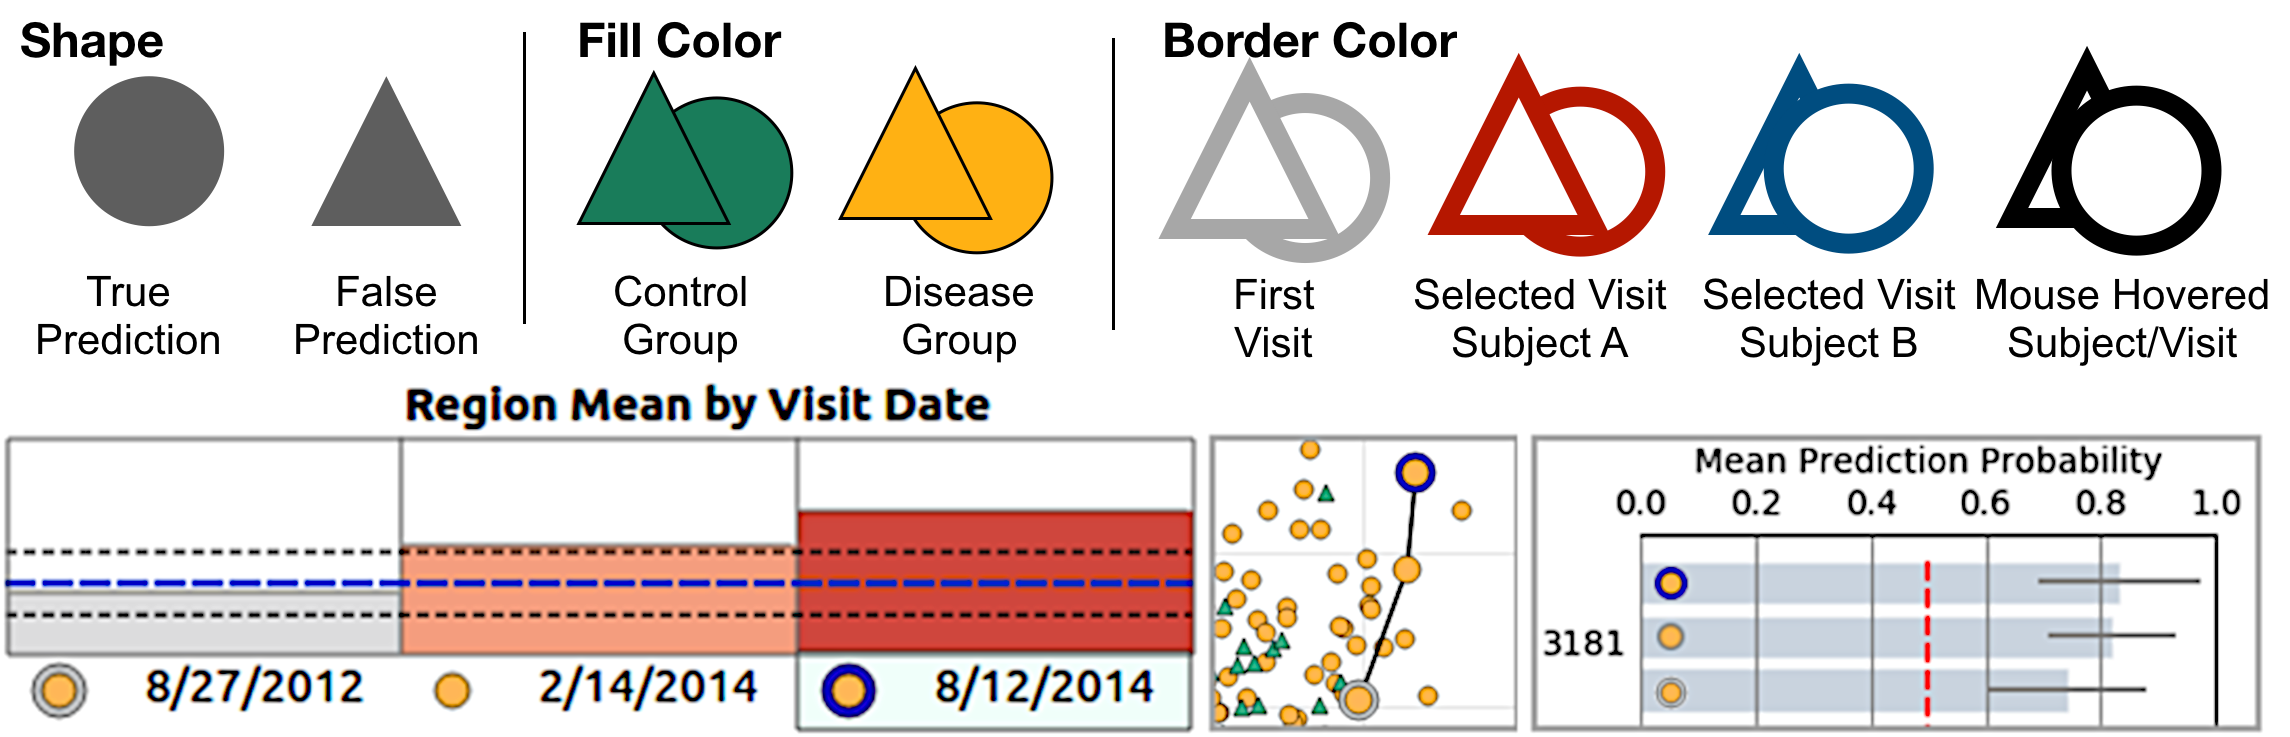
\includegraphics[width=1.0\textwidth]{images/pointEncoding.png}
% \caption{Glyph encoding. Shape encodes predicted class, fill color encodes true class, and the border distinguishes between pairs of selected subjects, and the temporal order of their different time-points (in conjunction with connecting lines for scatter plot views).}
% \label{fig:encoding}
% \end{figure}

\begin{figure}[tb]
\centering
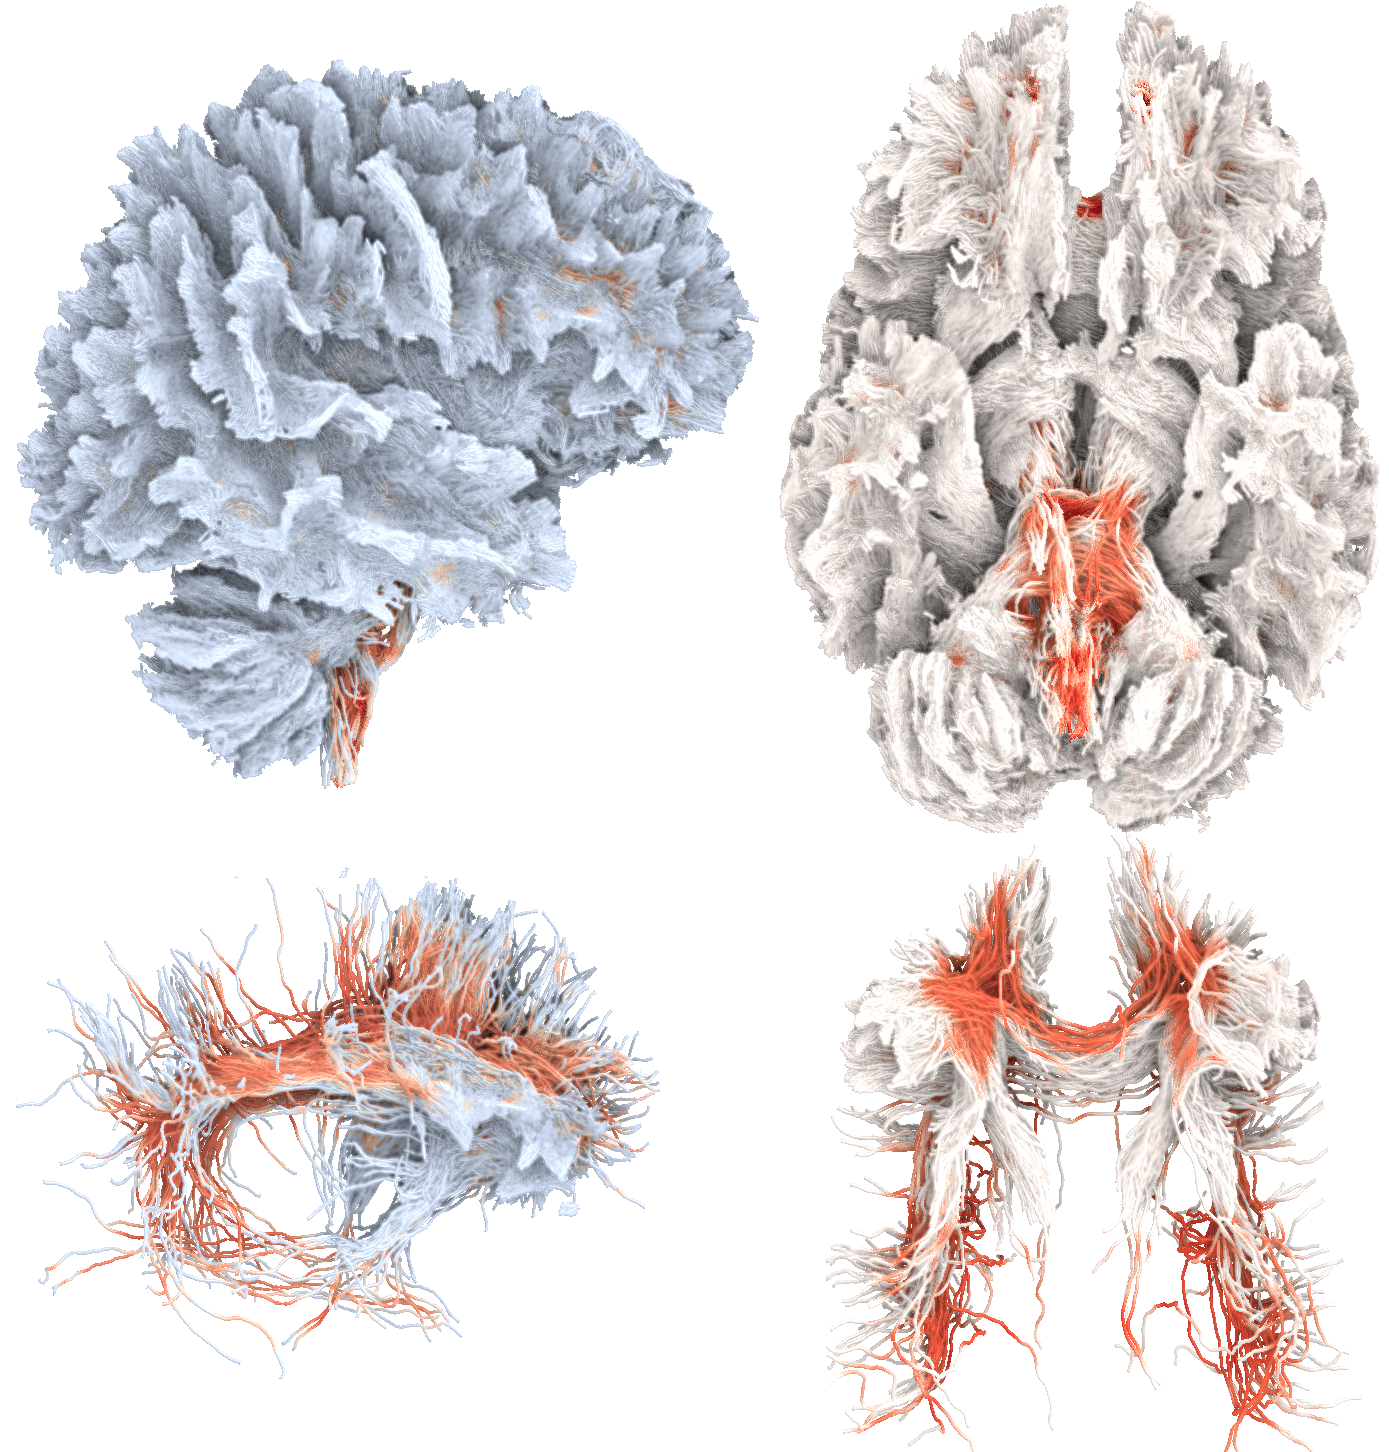
\includegraphics[width=0.99\textwidth]{rendering2.png}
\caption{Each column shows the whole brain and one bundle at the same orientation. SSAO rendering achieves a shadow effect that enhances spatial perception. (Left) diverging colors encode difference from the mean of the healthy group. (right) direct color mapping.}
\label{fig:rendering}
\end{figure}

\begin{figure*}[t]
\centering
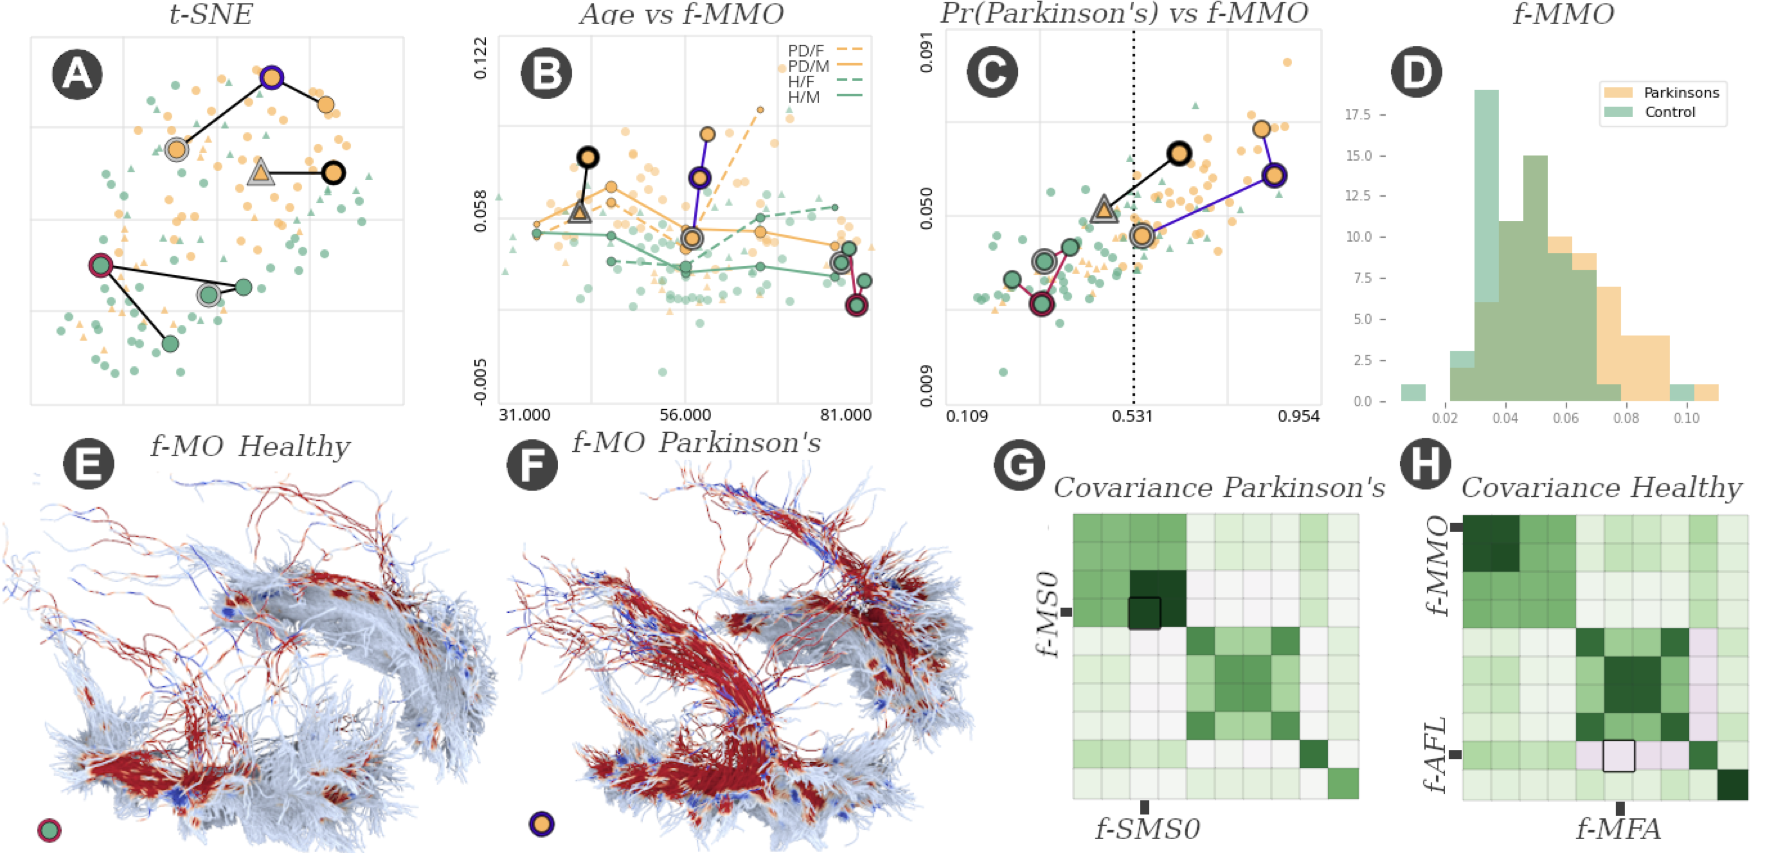
\includegraphics[width=0.99\textwidth]{images/comparisonV3labeled.png}
\caption{Visual comparisons in linked views (encodings are explained in Fig.~\ref{fig:subjectsUncertainty}). \glf{A} t-SNE plot using top 10 features with compared subjects highlighted. This view hints at multivariate similarity and ``community" structure.
\glf{B} Group trends in age vs mean mode of anisotropy (mean MO) in the fusiform region (f-MMO); dotted lines: female, solid lines: male, orange: PD, green: HC. \glf{C} Estimated probability of Parkinson's vs f-MMO. Dotted line shows the discrimination threshold (0.5). From this plot you can gain insight into the contribution of the salient feature to the classification model. You can then use the mouse to pick out subjects within the plot for various analysis directions. For example, select subjects that don't fit the group trend (e.g. correctly predicted PD subjects with low f-MMO), and then evaluate those subject's other features to better understand why the model predicted their class. \glf{D} Comparison of the distributions in f-MMO by group. This is a high level group comparison that gives instant insight into the group difference, and may also give insight into the statistical quality of the data. \glf{E},\glf{F} the fusiform fibers colored by the dis-aggregated MO values for the compared subjects The HC (left) and PD subject (right) are identified in the linked views by the green circle with red border, and orange circle with blue border respectively. \glf{G},\glf{H} Comparisons of the covariance for the top 10 features for the HC and the PD group respectively. Some interesting observations are pointed out: f-MMO (the salient feature) has higher variance in the Parkinson's group, and in bother groups is correlated positively with several other features. Second, a negative correlation between average fusiform fiber length (f-AFL) and mean fusiform fractional anisotropy (f-MFA) emerges for the Parkinson's group. Thirdly, there is a reduced overall in many of the features in the PD group compared with the healthy group. In the full user interface, the highlighted subjects are also shown in the time-point selection module, parallel coordinates view, and the subject exploration module as shown in Fig.~\ref{fig:system}, and Fig.~\ref{fig:subjectsUncertainty}.}
\label{fig:infovis}
\end{figure*}

\subsection{\textcolor{blue}{Visualizations and Interactions}}
\subsubsection{Fiber Rendering}
\label{sec:rendering}

\noindent The brain fibers are rendered (Fig.~\ref{fig:rendering}) as path tubes with screen space ambient occlusion (SSAO). This produces a high quality visualization with enhanced spatial perception that better shows fiber structure~\cite{mittring2007finding, eichelbaum2013lineao}. The path tubes are constructed on the fly through the GPU rendering pipeline in the geometry shader. This allows the pathtubes to be constructed and rendered quickly, with an interactively adjustable radius, and without additional memory overhead. The subjects, regions, and features (selected from their respective exploration modules) automatically determine which fibers are rendered, and which variables are used for color mapping.  User selected rendering options include: contrastive color mapping (which uses the difference from the mean value of the healthy group in order to emphasize anomaly), log scaling (which can better reflect subtle differences), and pathtube radius (which can help reduce or increase detail). These design decisions reflect \textbf{DG2} by providing a high quality visualize of fiber-microstructure with interactive frame-rates for large sets of brain fibers. 

https://www.overleaf.com/project/5f0699299304ab0001ca49c9
\begin{figure*}[t!]
\centering
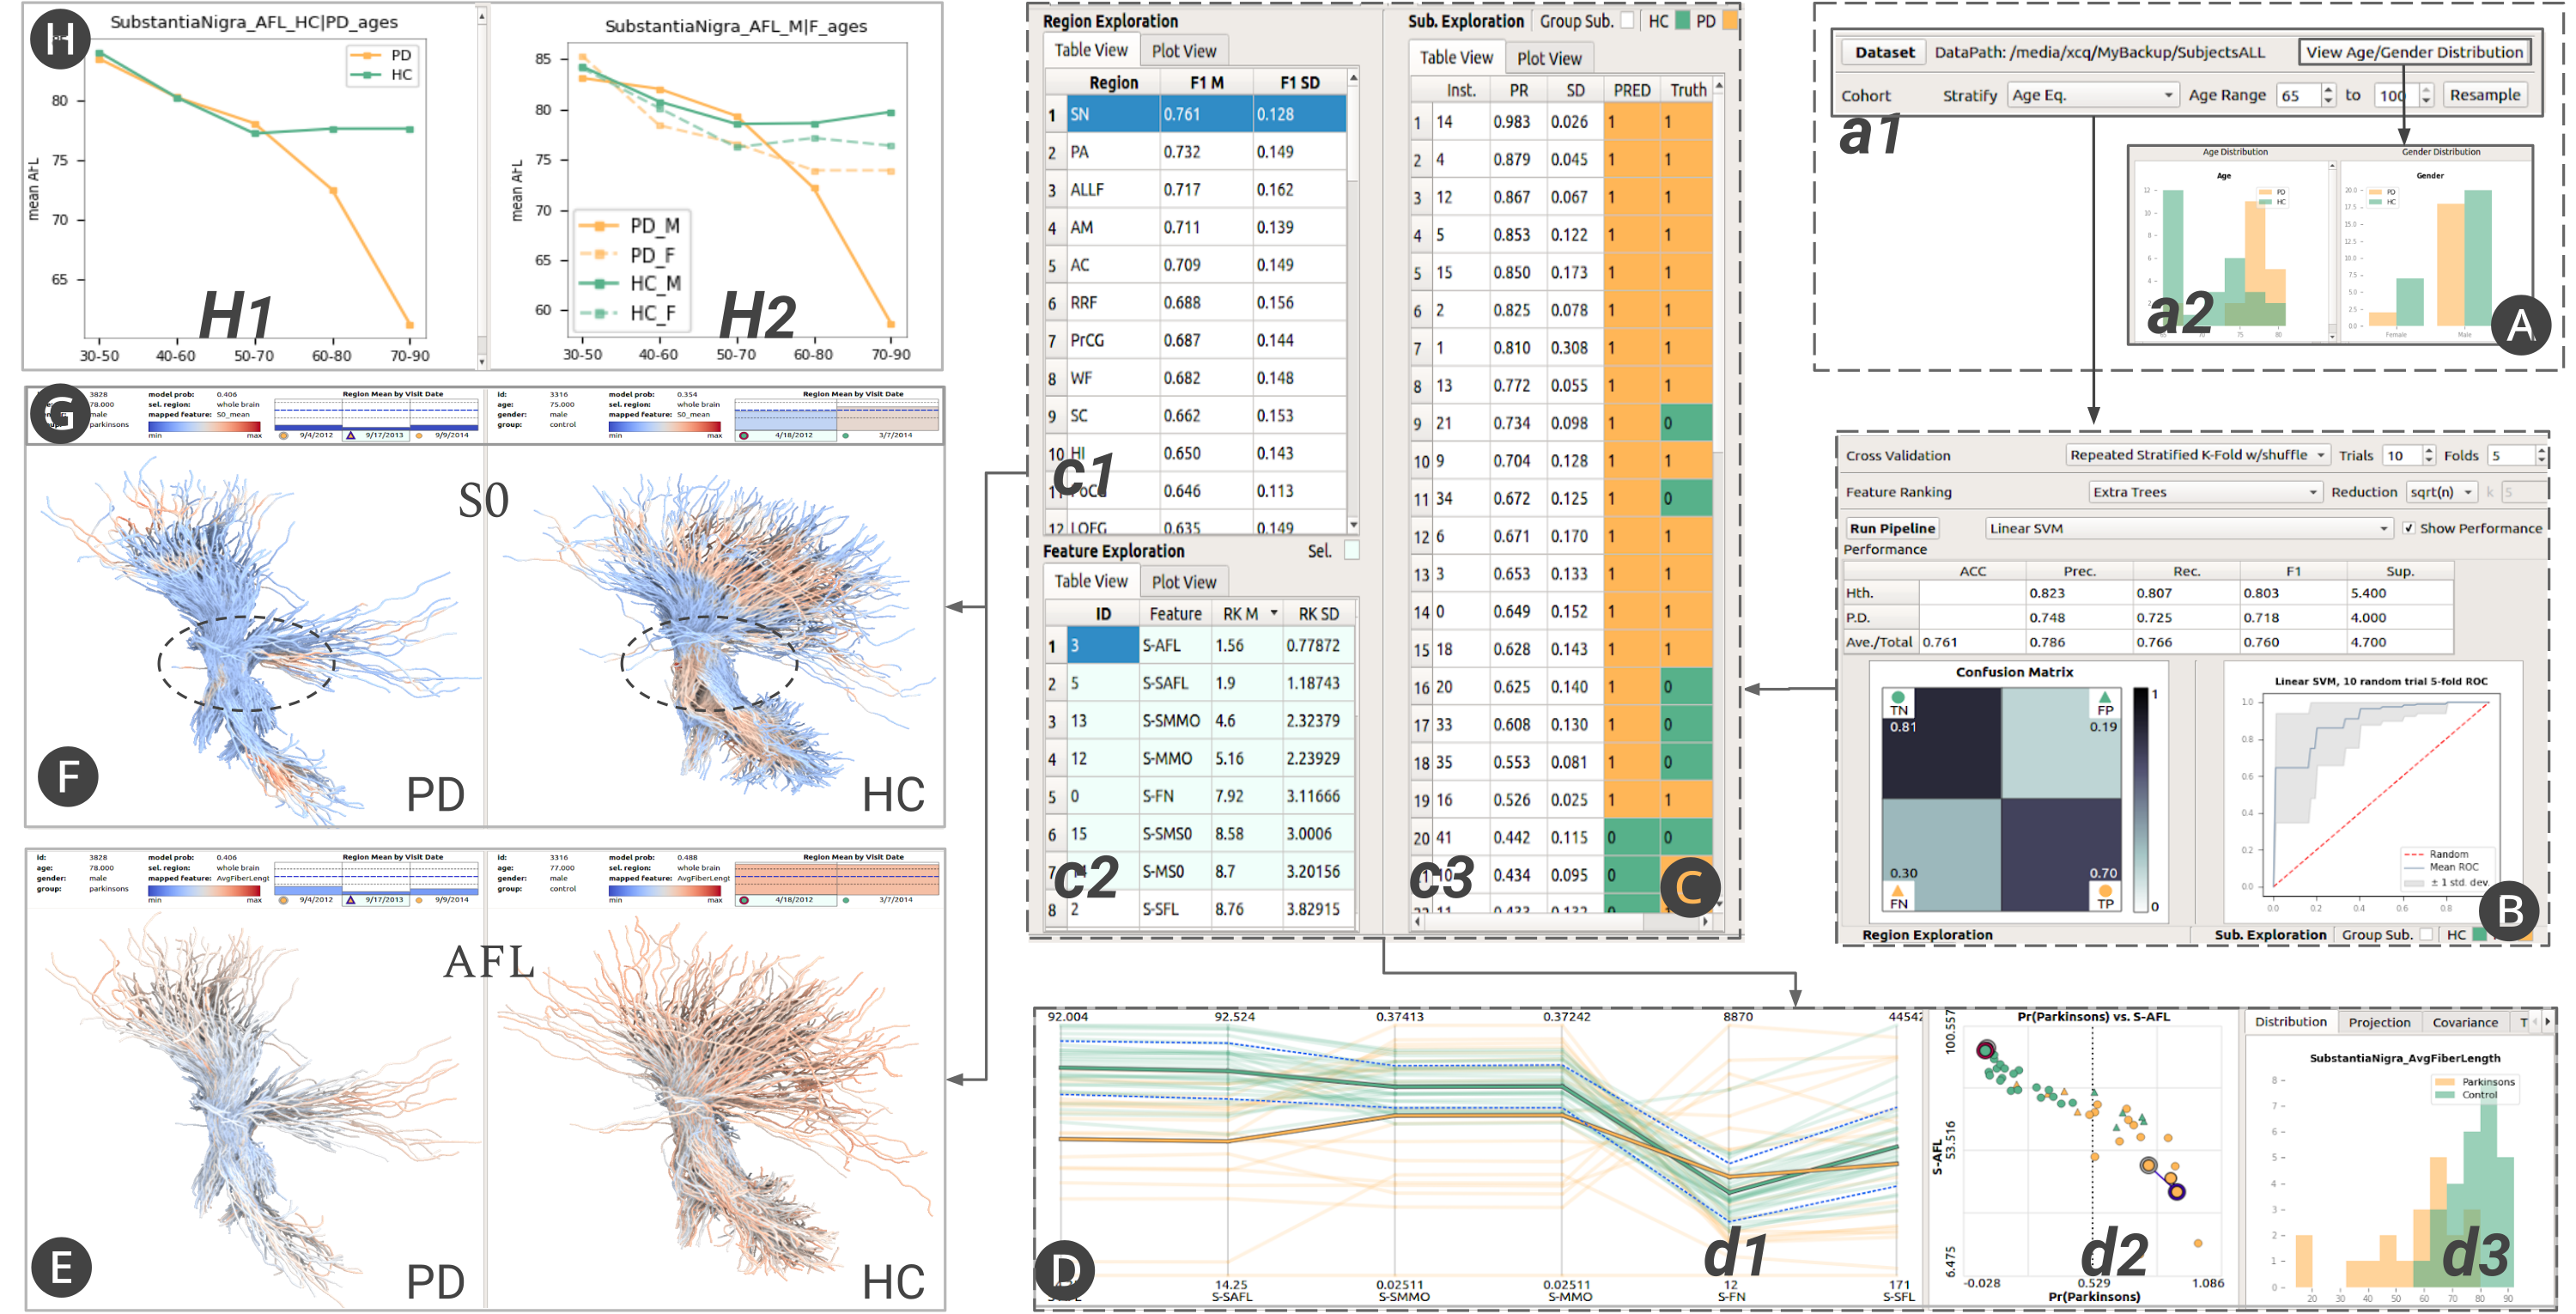
\includegraphics[width=0.98\textwidth]{images/SNSteps_v5.png}%
\caption{ Data selection module \glf{A}, entering an age range from \textbf{\textit{a1}} and displaying the distribution in \textbf{\textit{a2}}. ML module \glf{B}. users can run a ML algorithm with input parameters. Prediction results module \glf{C}. Brain regions \textbf{\textit{c1}}, features \textbf{\textit{c2}}, and subjects \textbf{\textit{c3}} were sorted in the table. Information visualization module \glf{D}. parallel coordinate \textbf{\textit{d1}}, partial dependence plot \textbf{\textit{d2}}, and bar chart \textbf{\textit{d3}} were used to show the distributions of the features and subjects. 3D rendering module \glf{E} and \glf{F}. Brain fibers were rendered in the juxta-positioned 3D rendering views for visual comparison with timeline views \glf{G}  of the selected subjects. Group trends plotting module \glf{H} ( trends with age \textbf{\textit{H1}} and trends with gender \textbf{\textit{H2}} ).}
\label{fig:SNSteps}
\end{figure*}


\subsubsection{Comparative Analysis}
\label{sec:comparison}

\noindent To support \textbf{DG3} we include a range of linked information visualization views that support a range of comparative modes for analysis. Besides the exploration modules, this includes: a histogram view, parallel coordinates view, scatter plot view, trend view, dimensionality reduction view, covariance matrix view, and subject time-point view. The views are linked with the exploration modules as shown in Fig.~\ref{fig:subjectsUncertainty}. The main aspects which are novel, are how they are customized to support the different modes of comparison for our application. We demonstrate by example in Fig.~\ref{fig:infovis}, and in the case studies in Sec.~\ref{sec:cases}. We reserve the rest of this section for some additional noteworthy details.  

Both covariance matrices and parallel coordinates can benefit from sorting to better highlight patterns~\cite{1382895}; in our case we apply hierarchical clustering to group correlated variables using the Louvain community detection algorithm~\cite{donetti2004detecting}. The same sorted order is applied to both views to assist the mental map~\cite{1215004}. The user can also switch from a covariance matrix to a correlation matrix.

Besides the information visualization views, the fiber views also incorporate design elements to facilitate comparison. First, the color map is scaled to be constant over all of visualized brains; after cohort selection, a global value range must be gathered over all subjects. Second, an option supports coloring the fibers by difference from the mean of the healthy control (HC) group. This supports comparison of the individuals against the HC, which may better emphasize important differences. The cameras between these views can also be linked so that they pan, rotate and zoom together. 

%One additional note, is that 
Uncertainty plays a major role in the workflows supported by our system. This begins with the overall model performance view (Fig.~\ref{fig:system} \clc{B}), which includes a receiver operating characteristics (ROC) curve. The ROC curve is used to assess the effect of prediction threshold on performance characteristics. In our case, we also highlight the variance of this curve over all CV trials, which is useful for assessing the overall sensitivity of the model to the training data. This is an important measure of uncertainty to consider during further comparative analysis. Once the user has made those assessments, they can collapse the view, to expand the sizes of the exploration module views. The variance each of the saliency measures is also included in the exploration modules (tables/plots) to make further assessment while exploring. These are important references to make while doing comparison, in order to avoid overconfidence and false insight.
